\chapter{Hacia un Framework Comparativo}
Android e iOS permiten cambiar ciertos permisos de una aplicación luego de haberla instalado en el dispositivo. En este contexto, se ha desarrollado un \textit{framework} para determinar empíricamente el alcance de dichos cambios en los sistemas de permisos de ambas plataformas.\\

El \textit{framework} es una aplicación móvil y está compuesto por varios tests. Cada test pone a prueba a un componente del dispositivo, permitiendo así conocer el alcance de los permisos correspondientes a dicho componente. De esta manera, se busca dejar en evidencia posibles vulnerabilidades presentes en los modelos de seguridad. Adicionalmente, se pone especial énfasis en la relación existente entre la privacidad del usuario y el sistema de permisos, analizando cuál es la cobertura del sistema respecto de los datos sensibles para la privacidad.\\

En las siguientes secciones se detallarán los distintos tests que componen el \textit{framework}. Además, se mencionarán las conclusiones arribadas luego de correr los tests mencionados anteriormente.
\section{Ejecución de los test}
Durante el momento de desarrollo de aplicaciones móviles multiplafoma, un desarrollador necesita tener los dispositivos reales para probar y depurar sus aplicaciones, hasta alcanzar el funcionamiento deseado. Sin embargo, a veces ocurre que el desarrollador no cuenta con todos los dispositivos en los que se ejecuta su aplicación. Es por ello que tanto Android como iOS proveen emuladores oficiales para salvar dicho inconveniente.\\

Los emuladores permiten interactuar de la misma manera que se haría con un dispositivo real, pero con el ratón y el teclado, y mediante los botones y los controles del emulador. De forma dinámica, permiten acercar y alejar la imagen, cambiar la orientación e, incluso, tomar una captura de pantalla. Además, son compatibles con pantallas táctiles y botones de \emph{hardware} virtuales, incluyendo también las operaciones con dos dedos.

Para el presente trabajo, se decidió utilizar los emuladores oficiales para testear el \emph{framework} propuesto. A continuación, se mencionan las principales características de los emuladores.
\subsection{Emulador oficial de Android}
Android provee un emulador para que un desarrollador pueda simular un dispositivo en la computadora de desarrollo. El emulador es compatible con teléfonos y tablets Android, y con dispositivos Android Wear y Android TV \cite{daemu}.\\

Cuando una aplicación se ejecuta en el emulador, puede usar los servicios de la plataforma Android para invocar otras aplicaciones, acceder a la red, almacenar y recuperar datos, y mostrar notificaciones. El emulador tiene controles que te permiten enviar mensajes de texto y llamadas telefónicas entrantes con facilidad, especificar la ubicación del dispositivo, simular lecturas de huellas digitales, y simular las propiedades de batería.\\

El emulador requiere una configuración de un AVD\footnote{Android Virtual Device, por sus siglas en inglés.} para determinar la apariencia, funcionalidad y versión del sistema del dispositivo simulado. Los AVD permiten definir determinados aspectos de \emph{hardware} de los dispositivos emulados. Cuentan con tipos de dispositivos predefinidos, como el teléfono Nexus, y permite crear definiciones propias. En la Figura \ref{fig:ch05:androidAVDsettings} se observa una captura del ADV utilizado para el desarrollo del \emph{framework}.
\begin{figure}[htbp]
    \centering
	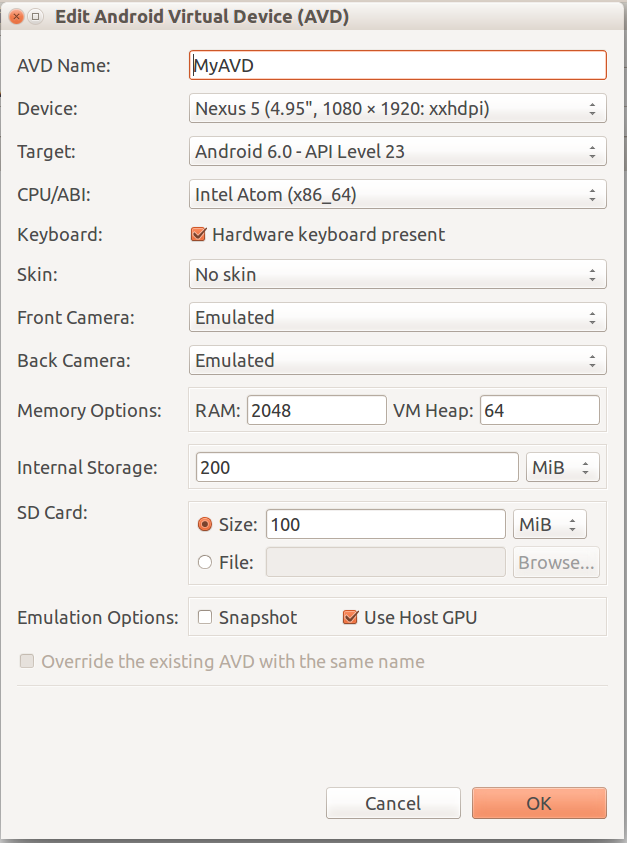
\includegraphics[width=.5\linewidth]{chapter4/android-AVD_settings}
	\caption{Configuración de un AVD.}
    \label{fig:ch05:androidAVDsettings}
\end{figure}
\subsection{Simulador oficial de iOS}
Apple provee un simulador, disponible dentro de Xcode, que se ejecuta como una aplicación independiente. El simulador presenta la interfaz de usuario de un iPhone, iPad, Apple Watch o Apple TV como una ventana en el escritorio de su Mac y le permite manipular esta pantalla y la aplicación que se ejecuta \cite{iosds}.\\

El simulador proporciona la capacidad de emular muchas combinaciones diferentes de tipo de dispositivo y versión de sistema operativo. Un tipo de dispositivo es un modelo de iPhone, iPad o Apple TV. Cada combinación de dispositivo-sistema operativo tiene su propio entorno de simulación con sus propias configuraciones y aplicaciones. También puede agregar simuladores para una combinación específica que quiera probar. Sin embargo, no todas las combinaciones de tipo de dispositivo y versión de SO están disponibles. Dicha configuración se realiza desde \texttt{Hardware/Dispositivo}.\\
\begin{figure}[tbp]
    \centering
	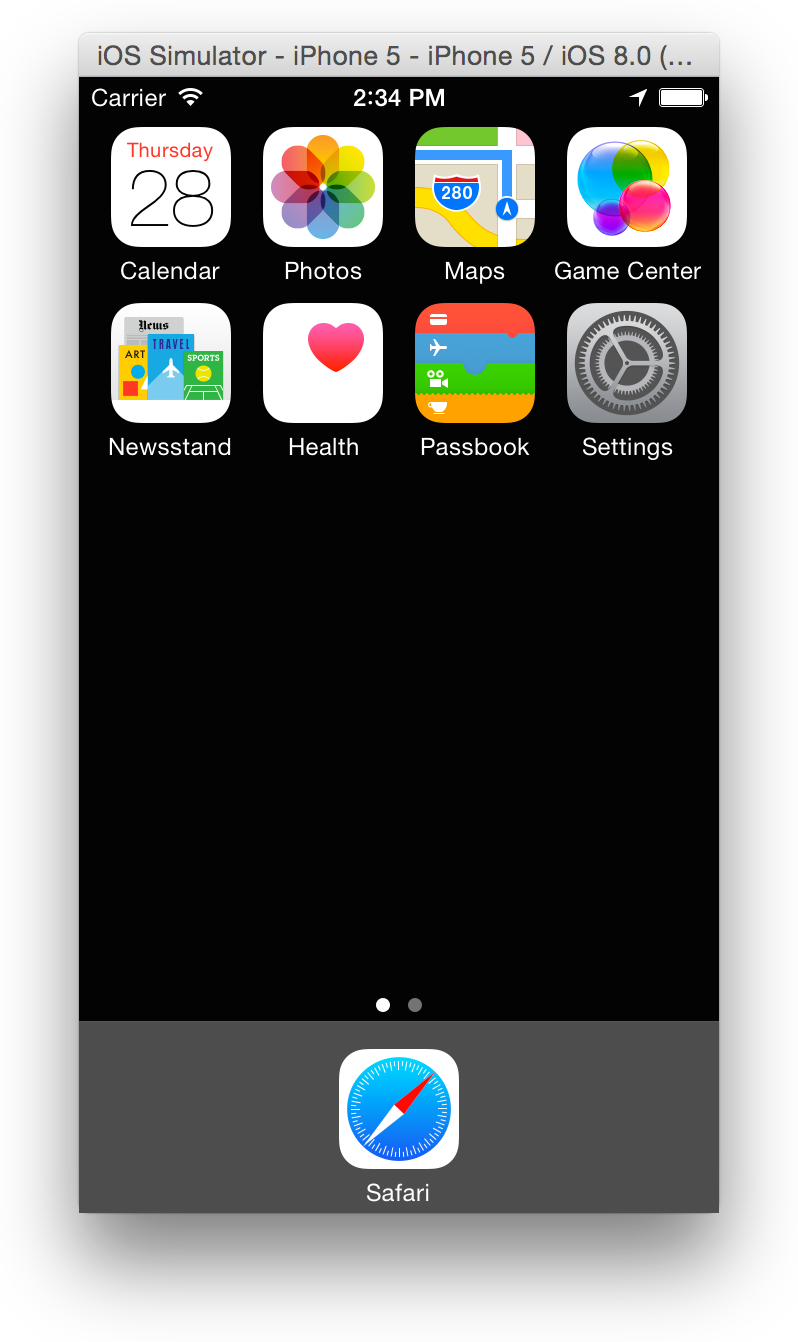
\includegraphics[width=.45\linewidth]{chapter5/ios-simulator-home}
	\caption{Pantalla de inicio del simulador de iOS \cite{iosds}.}
    \label{fig:ch05:ios-simulator-home}
\end{figure}

Para probar el funcionamiento de una aplicación, un desarrollador puede ejecutar su aplicación en el simulador directamente desde el proyecto de Xcode. El simulador proporciona herramientas para ayudarlo a depurar sus aplicaciones. Por ejemplo, se puede simular la ubicación dentro de una aplicación. En la Figura \ref{fig:ch05:ios-simulator-home} se observa el simulador emulando un iPhone 5 (iOS 8.0).\\

A pesar de todas las funcionalidades que provee, el simulador tiene sus limitaciones. No permite instalar aplicaciones desde App Store. Sumado a esto, muchas de las aplicaciones que vienen preinstaladas en dispositivos iOS no están disponibles en el simulador \cite{iosds}. Además, no todos los errores y problemas de rendimiento pueden detectarse mediante pruebas en el simulador.
\newpage
\section{Vista principal} \label{sec:main-view}
Al iniciar la aplicación se observan dos áreas principales: Acciones y Test, como se puede observar en la Figura \ref{fig:chapter05:main_view}.\\

La primera área contiene un botón para acceder a la configuración de los permisos del dispositivo. Allí, el \textit{tester} puede cambiar manualmente los permisos requeridos por la aplicación. Además, se encuentra un botón para limpiar la consola del \textit{framework}.\\

\begin{figure}[hbtp]
    \centering
	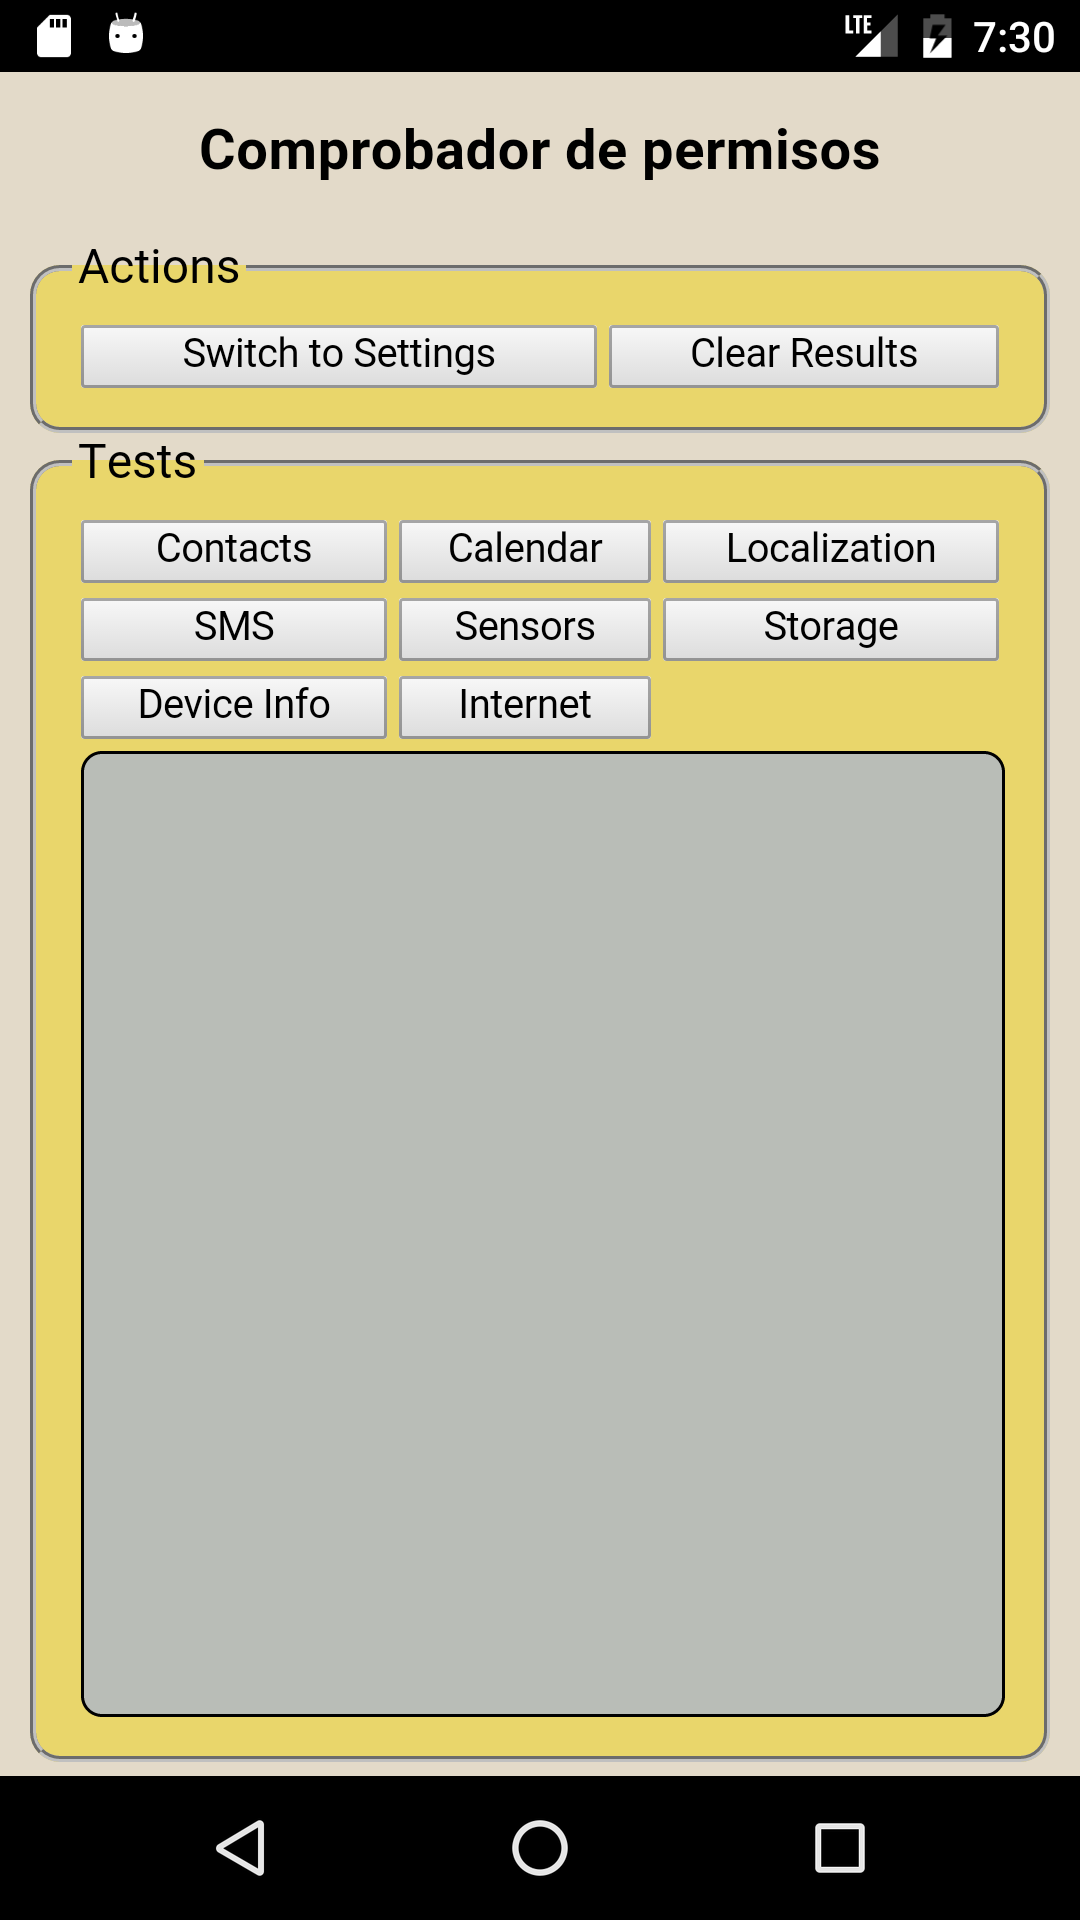
\includegraphics[width=0.4\linewidth]{chapter5/app_main_view}
	\caption{Áreas del \textit{framework}.}
	\label{fig:chapter05:main_view}
\end{figure}
La segunda área se subdivide en dos: la parte de los tests y la parte de la consola. Una parte contiene un conjunto de botones que, al presionarse, ejecutan un test. El resultado se imprimirá en la consola con tipografía color verde si fue exitoso; en cambio, se imprimirá con tipografía color roja de si falla.\\

A continuación se mencionan los componentes que se pueden testear con el \textit{framework}:
\begin{itemize}
	\item Contactos
	\item Calendario
	\item Geolocalización
	\item SMS
	\item Sensores
	\item Almacenamiento
	\item Información del dispositivo
	\item Acceso a Internet
\end{itemize}
\subsection{Funciones no compatibles}
El emulador oficial de Android es compatible con la mayoría de las funciones de un dispositivo, pero no incluye la posibilidad de virtualizar los siguientes componentes \cite{daemu}:
\begin{itemize}
    \item WiFi
    \item Bluetooth
    \item NFC\footnote{Del ingles \emph{Near Field Communication}. Es una tecnología de comunicación inalámbrica, de corto alcance y alta frecuencia que permite el intercambio de datos entre dispositivos.}
    \item Manipulación de la tarjeta SD
    \item Conexión USB
    \item Micrófono
    \item Cámara
\end{itemize}
Al no poder manipular la tarjeta SD, no es posible testear las funcionalidades multimedia: no se puede grabar audio, ni video ni sacar fotos. Por lo tanto, no se agregaron al \textit{framework} tests para los componentes listados anteriormente.
\section{Catálogo de Tests}
En esta sección se listarán todos los test que conforman el \textit{framework}. Para cada uno de ellos se detalla el algoritmo, los plugins de Apache Cordova que se utilizaron para desarrollarlo y una serie de capturas que muestran los casos exitosos y fallidos.\\

Para acceder al panel de configuraciones, se utilizó el \textit{plugin} \href{https://www.npmjs.com/package/cordova.plugins.diagnostic}{cordova.plugins.diagnostic (v. 3.0.4)} de Apache Cordova.\\

De ahora en adelante, cuando se diga `consola', se refiere a la consola del \textit{framework}.
\subsection{Contactos}
\begin{algorithm}
	\begin{algorithmic}[1]
		\STATE Se imprimen por consola todos los contactos.
		\STATE Se crea un nuevo contacto.
		\STATE Se vuelven a imprimir por consola todos los contactos.
	\end{algorithmic}
	\caption{Test de Contactos.}\label{alg:chap5:test_contactos}
\end{algorithm}
El test consiste en crear un contacto y luego listar todos los contactos presentes en el dispositivo. En caso de ser exitoso, se imprimen los contactos por consola. De lo contrario, se imprime un error. En la Figura \ref{fig:ch05:without_contact} se observa el resultado del test cuando no se tiene el permiso correspondiente; mientras que en la Figura \ref{fig:ch05:with_contact} se observa el caso exitoso.\\

Para desarrollarlo, se utilizó el \textit{plugin} \href{https://www.npmjs.com/package/cordova-plugin-contacts}{cordova-plugin-contacts (v. 2.3.1)} de Apache Cordova.\\

Finalmente, para correr el test, es necesario tener el permiso \texttt{Contacto}, tanto para Android como para iOS.
\begin{figure}[htbp]
    \centering
    \begin{subfigure}{0.3\linewidth}
        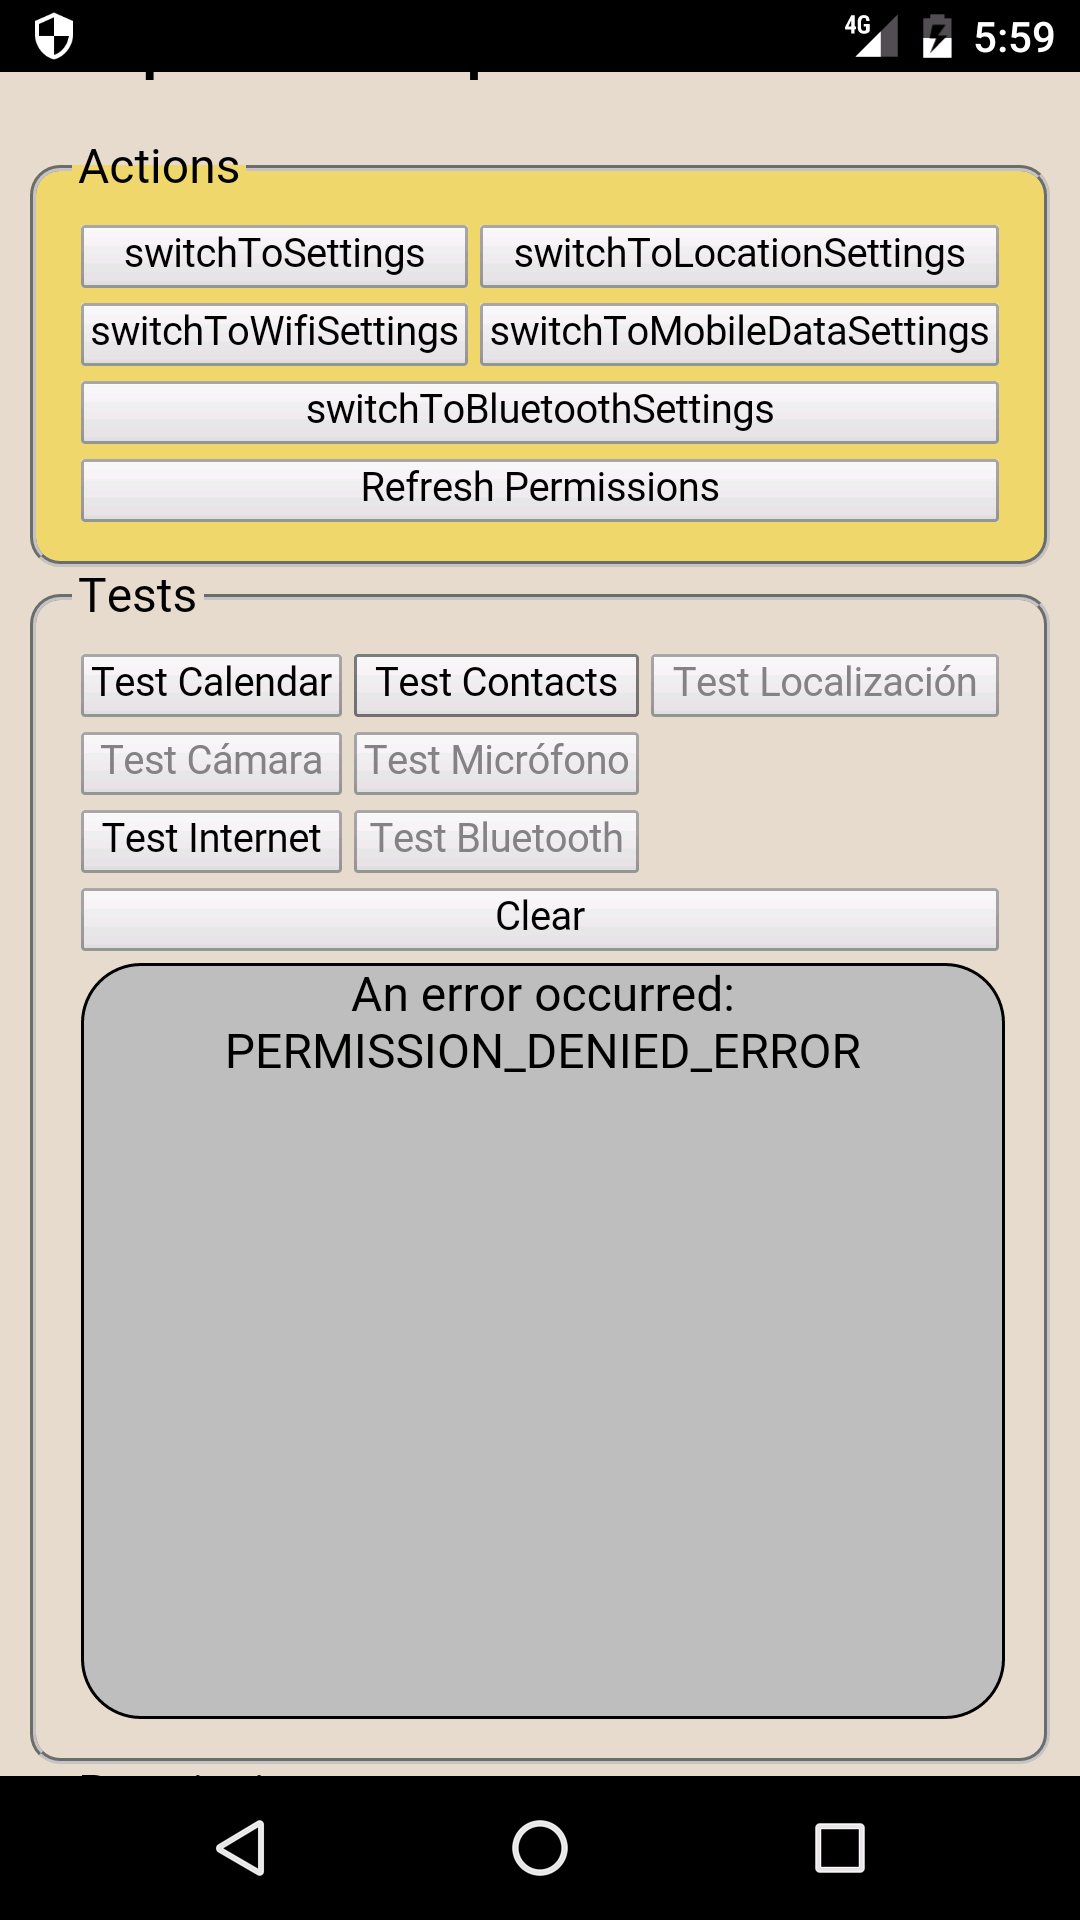
\includegraphics[width=\linewidth]{chapter5/without_contact}
        \caption{Sin permisos.}
        \label{fig:ch05:without_contact}
    \end{subfigure}
    \begin{subfigure}{0.3\linewidth}
        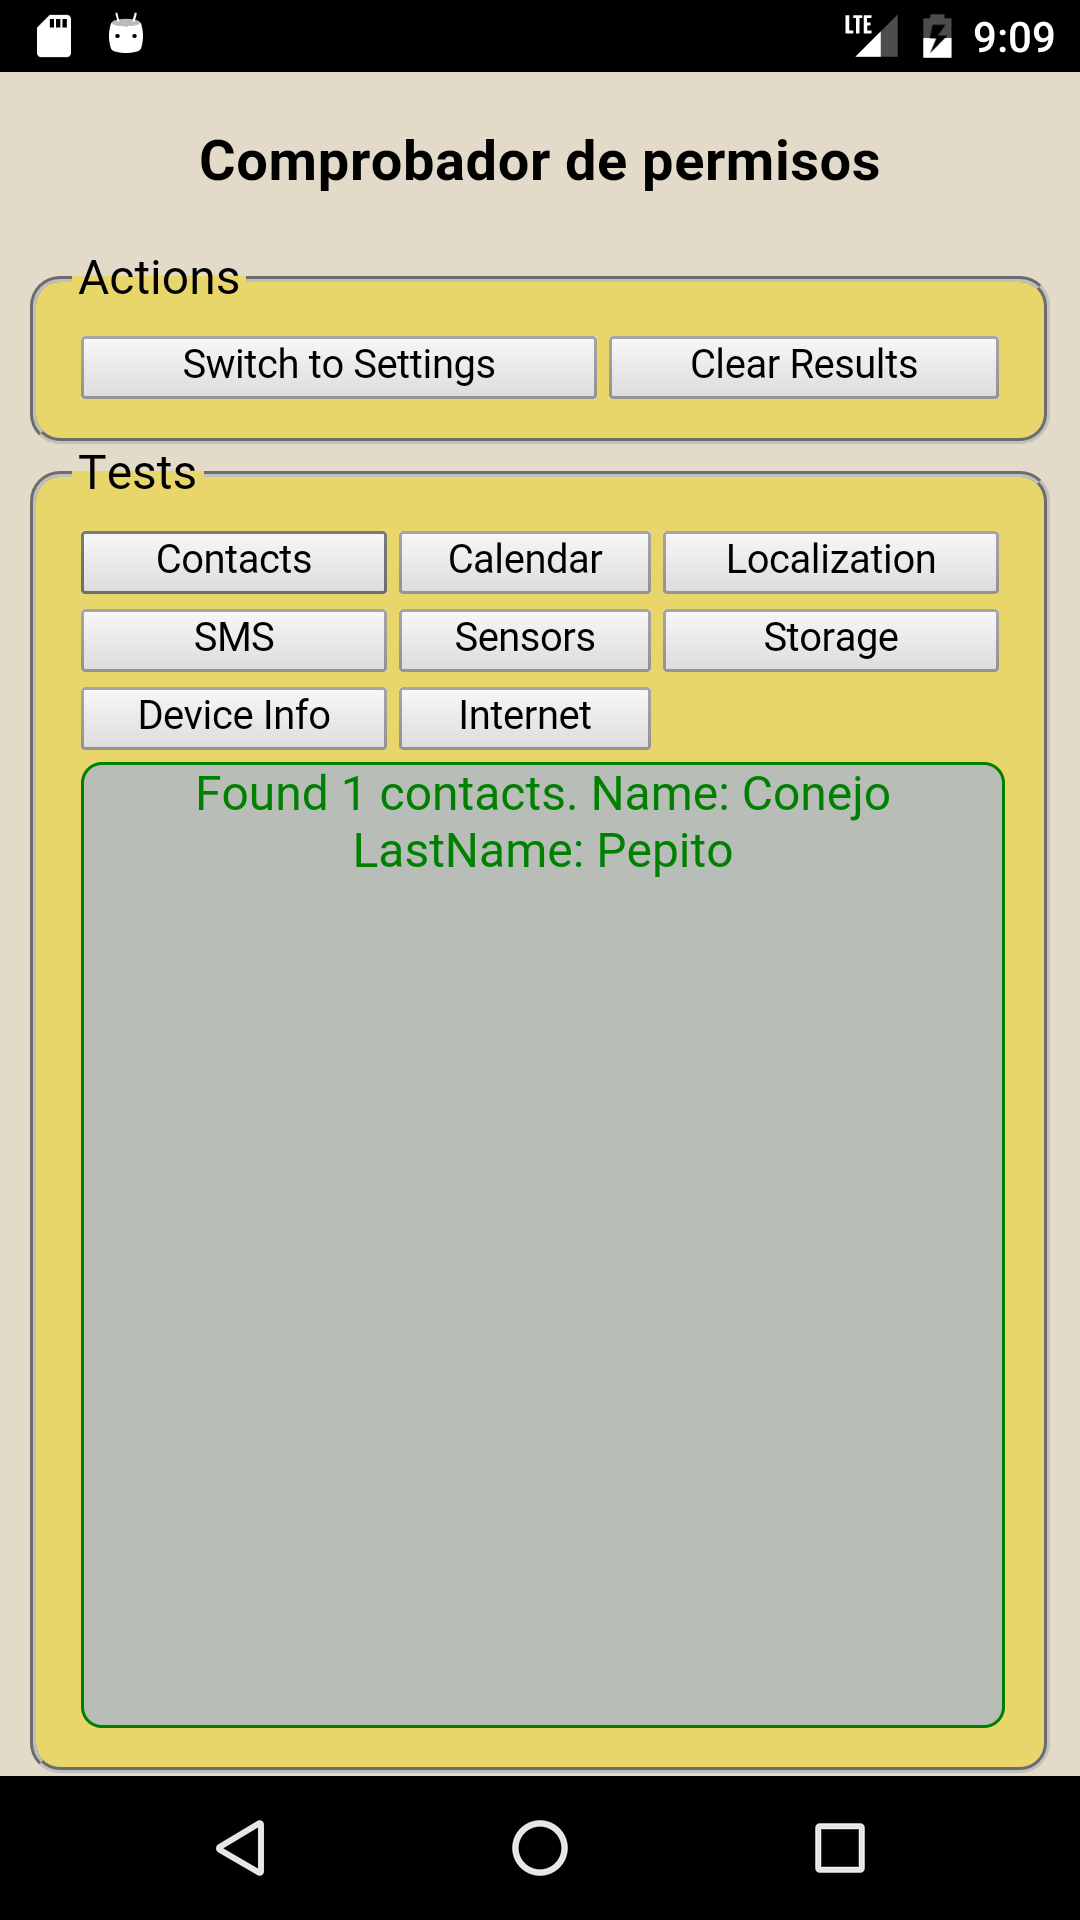
\includegraphics[width=\linewidth]{chapter5/with_contact}
        \caption{Con permisos.}
        \label{fig:ch05:with_contact}
    \end{subfigure}
    \caption{Testeando la administración de los contactos.}
	\label{fig:ch05:contacts-cases}
\end{figure}
\subsection{Calendario}
\begin{algorithm}
	\begin{algorithmic}[1]
		\STATE Se crean las fechas $startDate$ y $endDate$.
		\STATE Se crea un evento que empieza en la fecha $startDate$ y termina en la fecha $endDate$.
		\STATE Se imprimen por consola los eventos entre las fechas $startDate$ y $endDate$.
	\end{algorithmic}
	\caption{Test del Calendario.}\label{alg:chap5:test_calendario}
\end{algorithm}
El test consiste en crear un evento en un determinado rango de fechas y luego listar todos los eventos dentro del rango. En caso de ser exitoso, se muestran los datos del evento. De lo contrario, se muestra un error. En la Figura \ref{fig:ch05:without_calendar} se observa el resultado del test cuando no se tiene el permiso correspondiente; mientras que en la Figura \ref{fig:ch05:with_calendar} se observa el caso exitoso.\\

Para desarrollarlo, se utilizó el \textit{plugin} \href{https://www.npmjs.com/package/cordova-plugin-calendar}{cordova-plugin-calendar (v. 4.6)} de Apache Cordova.\\

Finalmente, para correr el test, es necesario tener el permiso \texttt{Calendario} para Android. En cambio, para iOS, es necesario tener el permiso \texttt{Recordatorios}.
\begin{figure}[tp]
    \centering
    \begin{subfigure}{0.3\linewidth}
        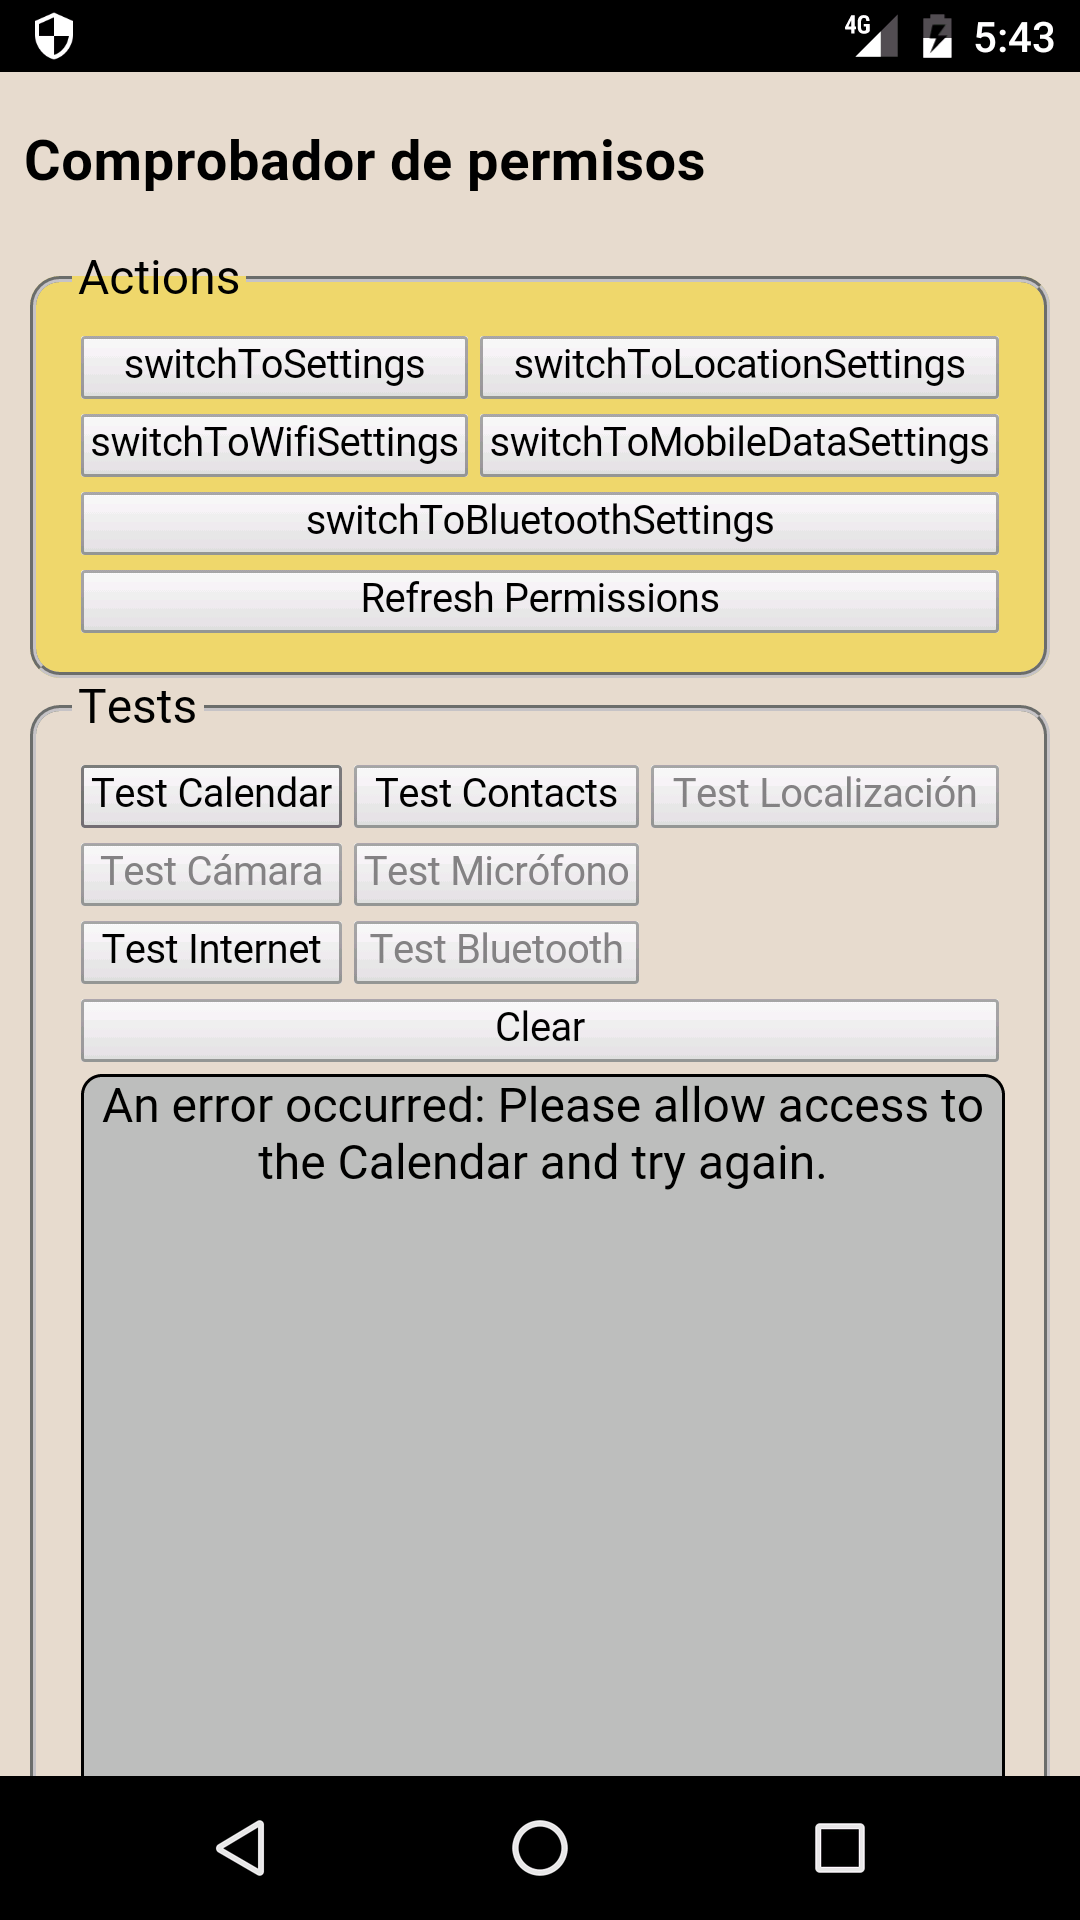
\includegraphics[width=\linewidth]{chapter5/without_calendar}
        \caption{Sin permisos.}
        \label{fig:ch05:without_calendar}
    \end{subfigure}
    \begin{subfigure}{0.3\linewidth}
        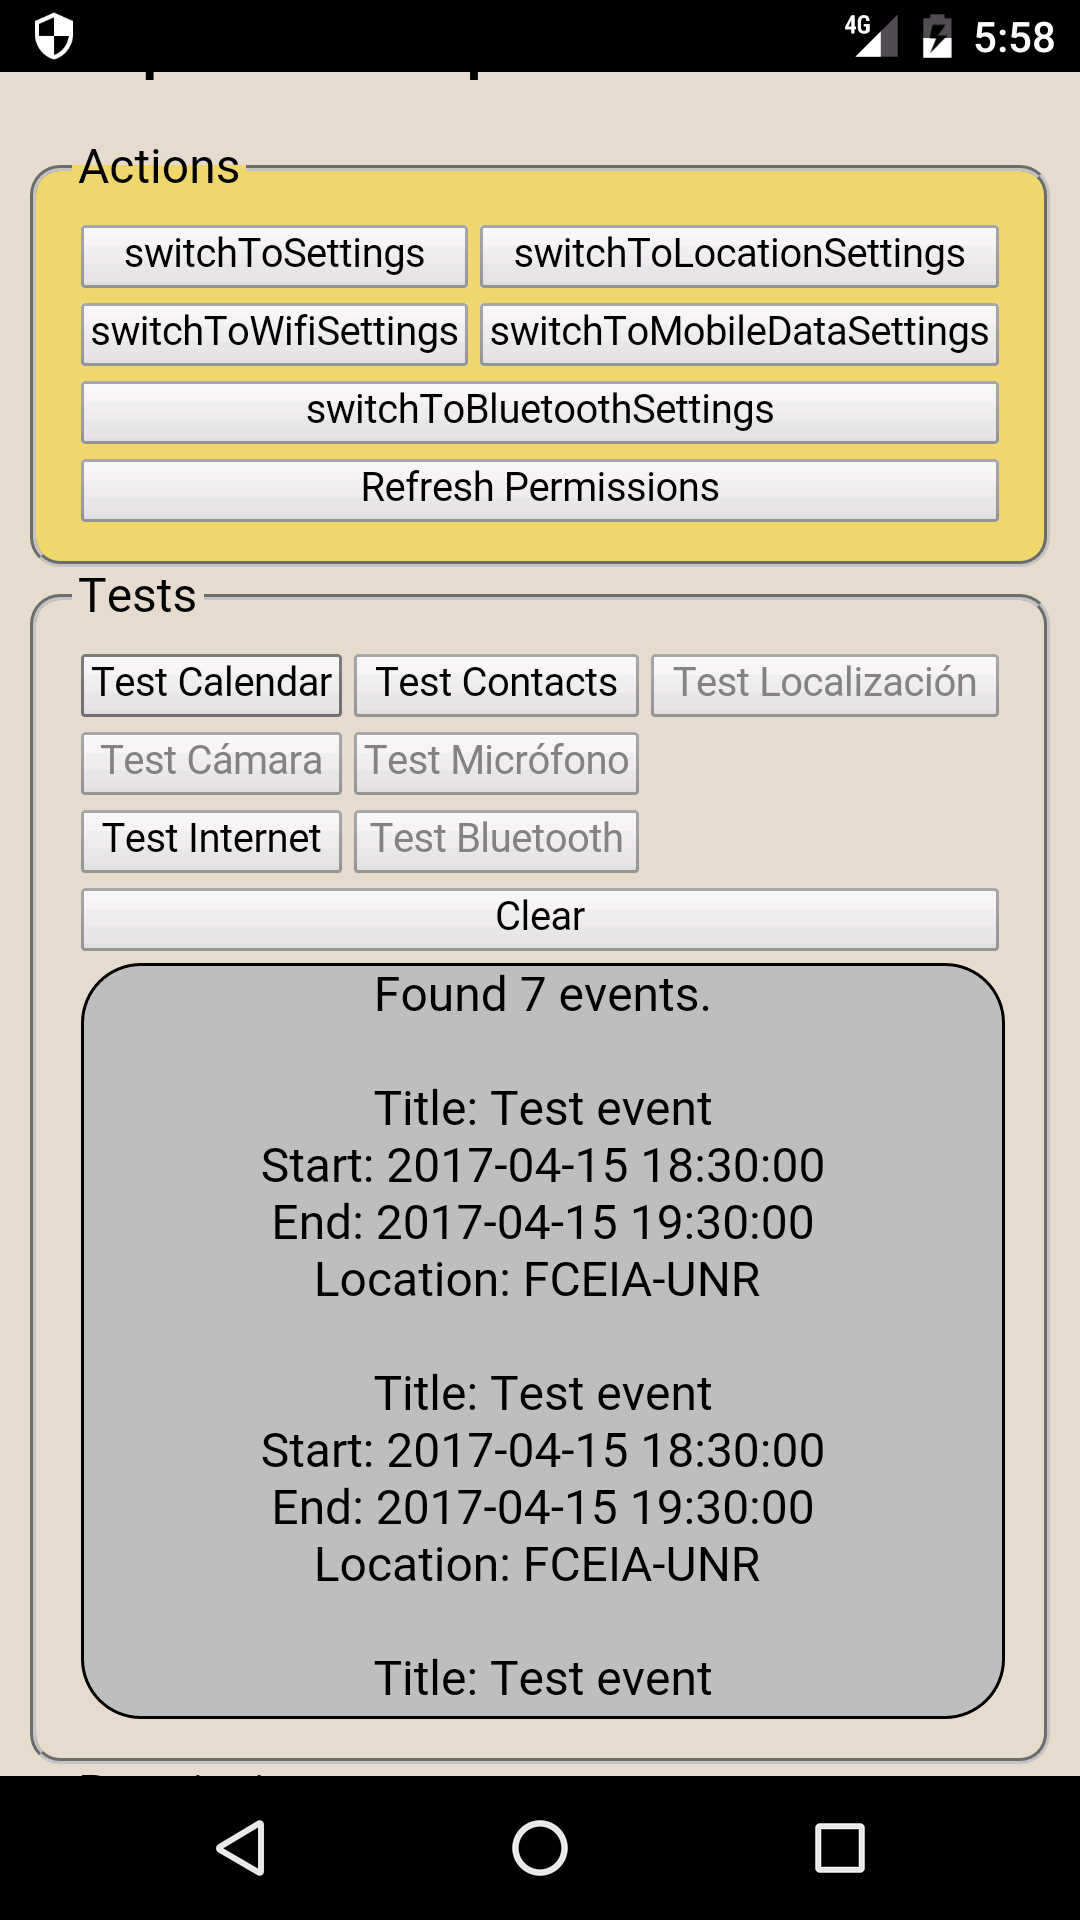
\includegraphics[width=\linewidth]{chapter5/with_calendar}
        \caption{Con permisos.}
        \label{fig:ch05:with_calendar}
    \end{subfigure}
    \caption{Testeando la administración del calendario.}
	\label{fig:ch05:calendar-cases}
\end{figure}
\newpage
\subsection{Geolocalización}
\begin{algorithm}
	\begin{algorithmic}[1]
		\STATE Se censa el GPS.
		\STATE Se imprimen por consola los datos.
	\end{algorithmic}
	\caption{Test de Geolocalización.}\label{alg:chap5:test_geolocalizacion}
\end{algorithm}
El objetivo del presente test es obtener los datos de la ubicación actual. En caso de tener los permisos correspondientes, obtiene tanto la ubicación precisa (GPS) como la aproximada (WIFI/Móvil). En la Figura \ref{fig:ch05:without_location} se observa el resultado del test cuando no se tiene el permiso correspondiente; mientras que en la Figura \ref{fig:ch05:with_location} se observa el caso exitoso.\\

Para desarrollarlo, se utilizó el \textit{plugin} \href{https://github.com/apache/cordova-plugin-geolocation}{cordova-plugin-geolocation (v. 2.4.3)} de Apache Cordova.\\

Al momento de realizar las pruebas, se configuró el emulador de Android para que simule las coordenadas \texttt{(-122$^\circ$, 37$^\circ$)}, tal como se observa en la Figura \ref{fig:ch05:android_extended_controls}. Dicha configuración también se realizo en emulador oficial de iOS.\\

Finalmente, para correr el test, es necesario tener el permiso \texttt{Localización}, tanto para Android como para iOS.
\begin{figure}[htbp]
    \centering
	\begin{subfigure}{0.3\linewidth}
		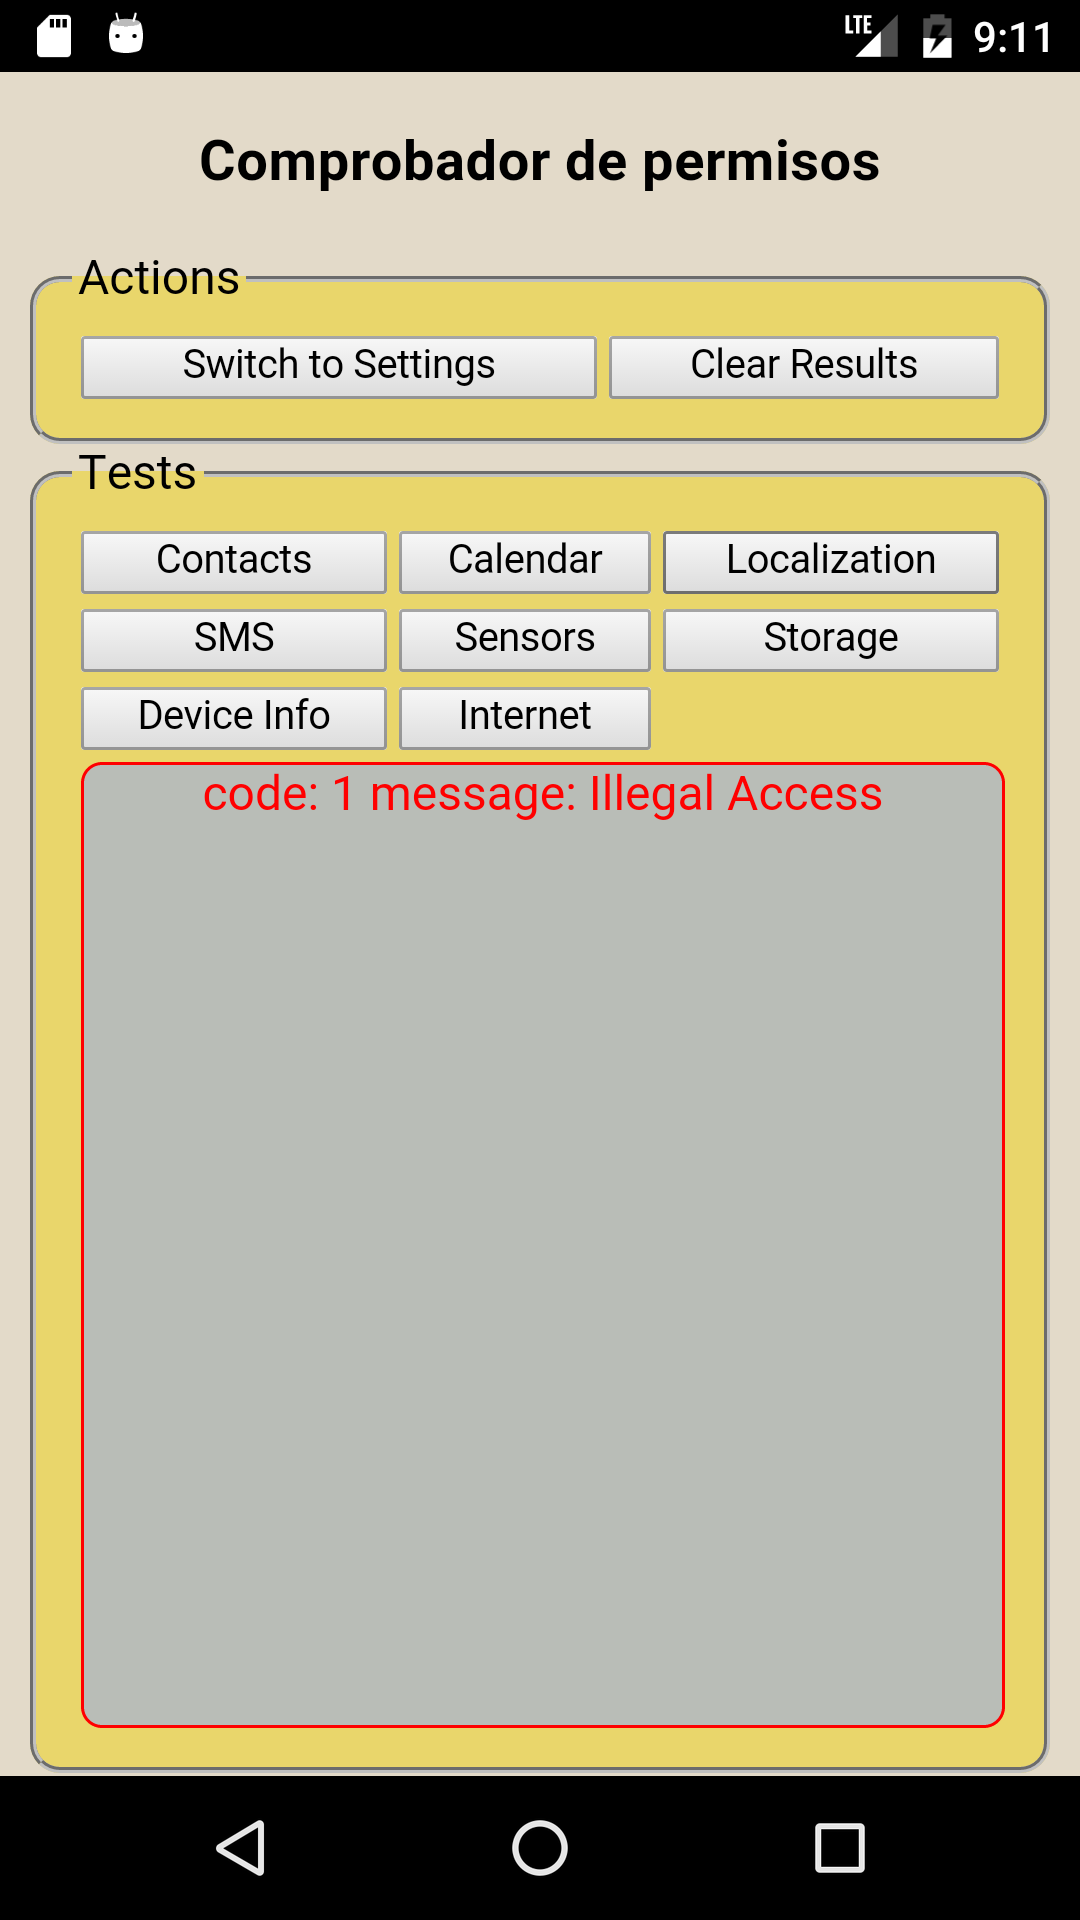
\includegraphics[width=\linewidth]{chapter5/without_location}
		\caption{Sin permisos.}
		\label{fig:ch05:without_location}
	\end{subfigure}
	\begin{subfigure}{0.3\linewidth}
		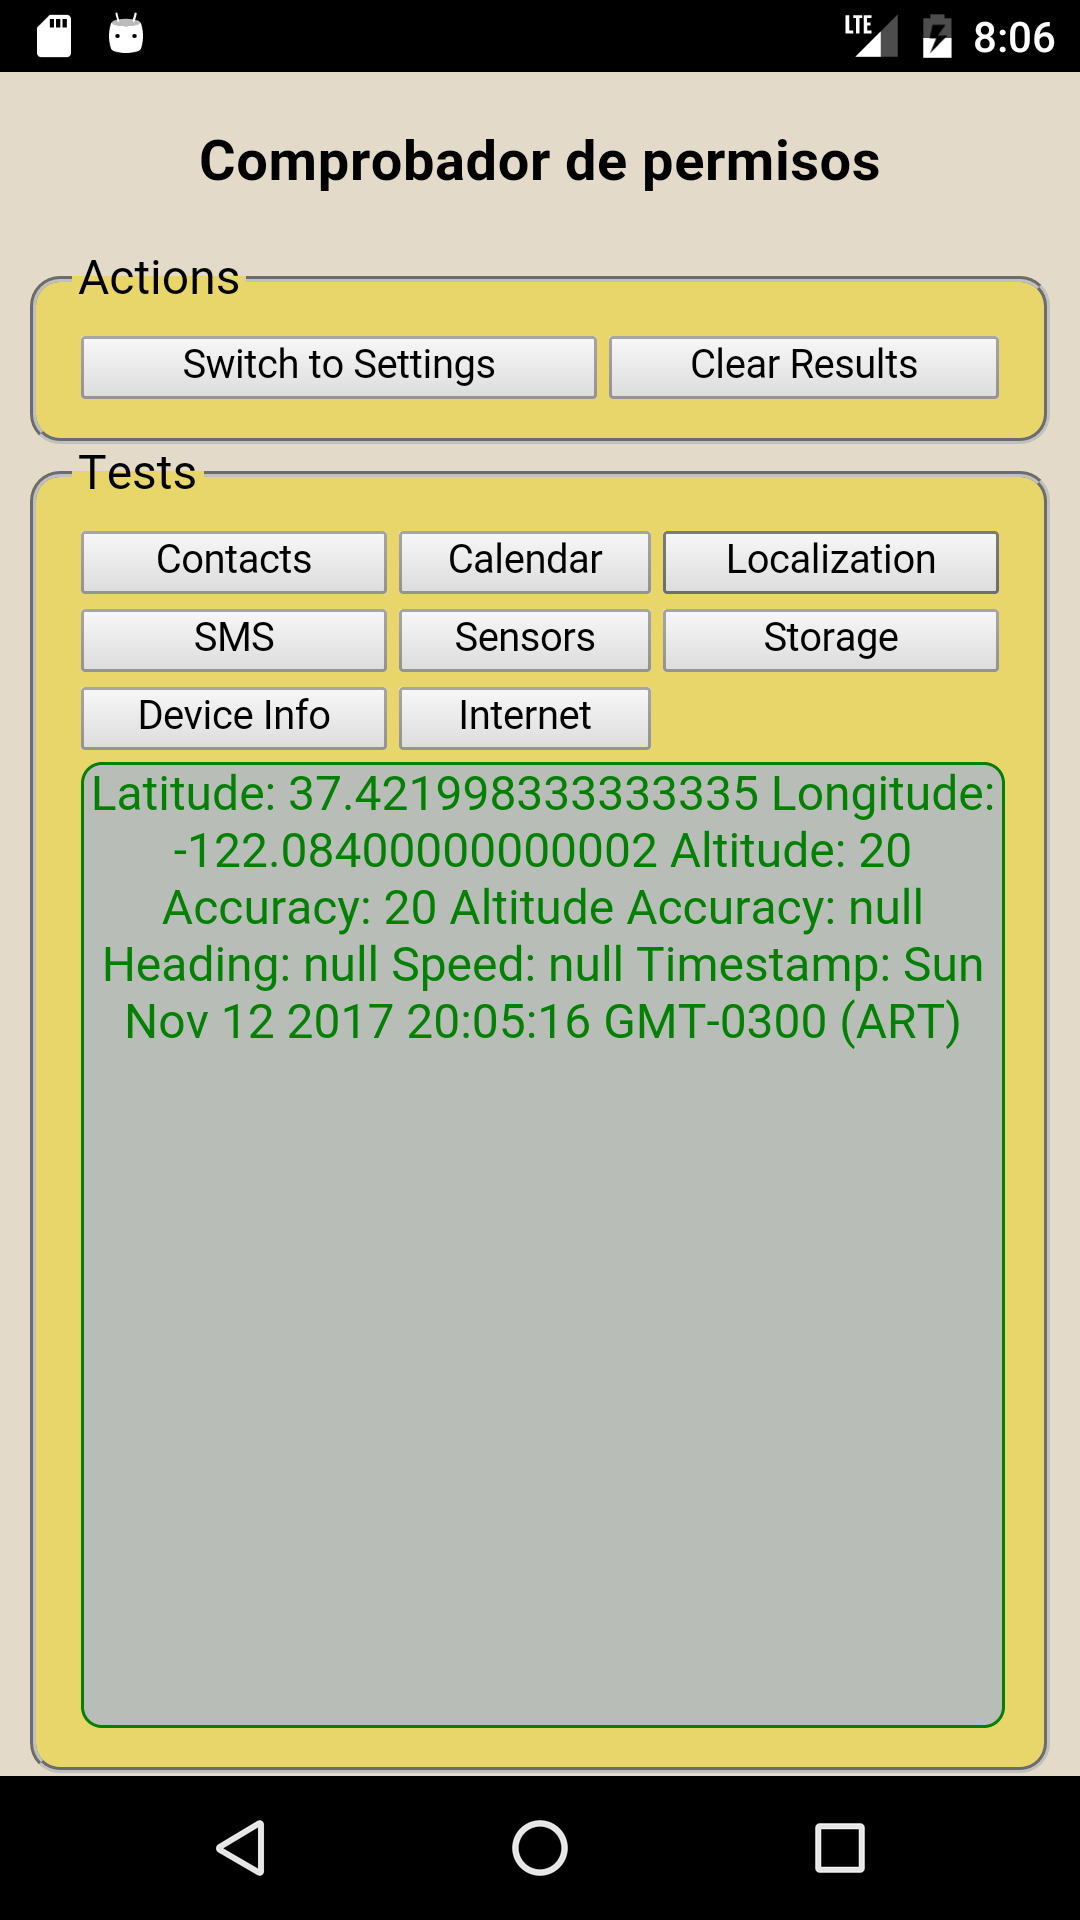
\includegraphics[width=\linewidth]{chapter5/location_success}
		\caption{Con permisos.}
		\label{fig:ch05:with_location}
	\end{subfigure}
	\caption{Testeando la geolocalización.}
	\label{fig:ch05:geolocation-cases}
\end{figure}
\begin{figure}[hbtp]
    \centering
	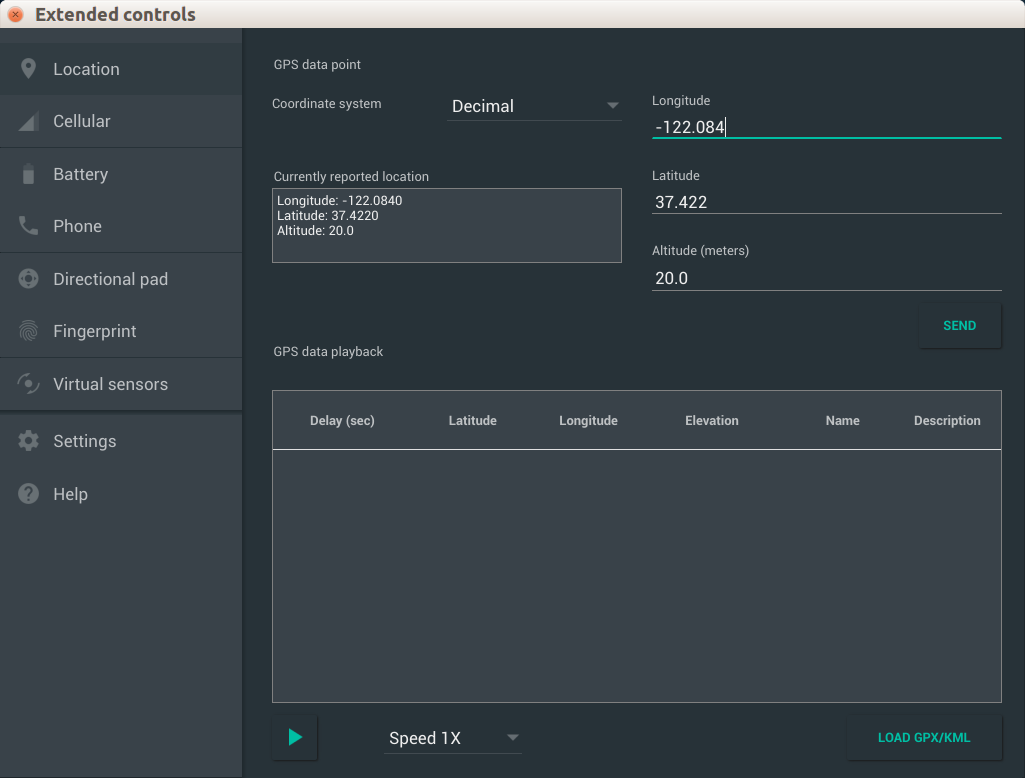
\includegraphics[width=0.65\linewidth]{chapter5/android_extended_controls}
	\caption{Panel de configuración del emulador de Android.}
	\label{fig:ch05:android_extended_controls}
\end{figure}
\newpage
\subsection{SMS}
\begin{algorithm}
	\begin{algorithmic}[1]
		\STATE Se envía un SMS de prueba.
		\STATE Se imprime por consola el resultado del test.
	\end{algorithmic}
	\caption{Test de SMS.}
	\label{alg:chap5_test_sms}
\end{algorithm}
El test consiste en enviar un mensaje SMS. En un principio, se diseñó con la capacidad de enviar, leer y recibir mensajes. Al momento de desarrollarlo, se encontró una restricción de seguridad en iOS: a partir de la version 8 no se pueden acceder a los mensajes SMS desde una aplicación instalada por el usuario \cite{foda, foda2}. En cambio, en Android sí se pueden acceder, siempre que se tengan el permiso correspondiente. Dicho permiso permiso es \texttt{SMS}.\\

Como consecuencia de lo mencionado en el párrafo anterior, se decidió no implementar las funcionalidades incompatibles, quedando en el test la posibilidad de enviar mensajes SMS. Para desarrollarlo, se utilizó el \textit{plugin} \href{https://github.com/floatinghotpot/cordova-plugin-sms}{cordova-plugin-sms (v. 0.1.11)} de Apache Cordova.\\

En la Figura \ref{fig:ch05:without_sms} se observa el resultado del test cuando no se tiene el permiso correspondiente; mientras que en la Figura \ref{fig:ch05:with_sms} se observa el caso exitoso.\\
Finalmente, para correr el test, es necesario tener el permiso \texttt{SMS} para Android. Sin embargo, no es necesario tener permisos para correr el test en iOS.
\begin{figure}[hbtp]
    \centering
	\begin{subfigure}{.3\linewidth}
		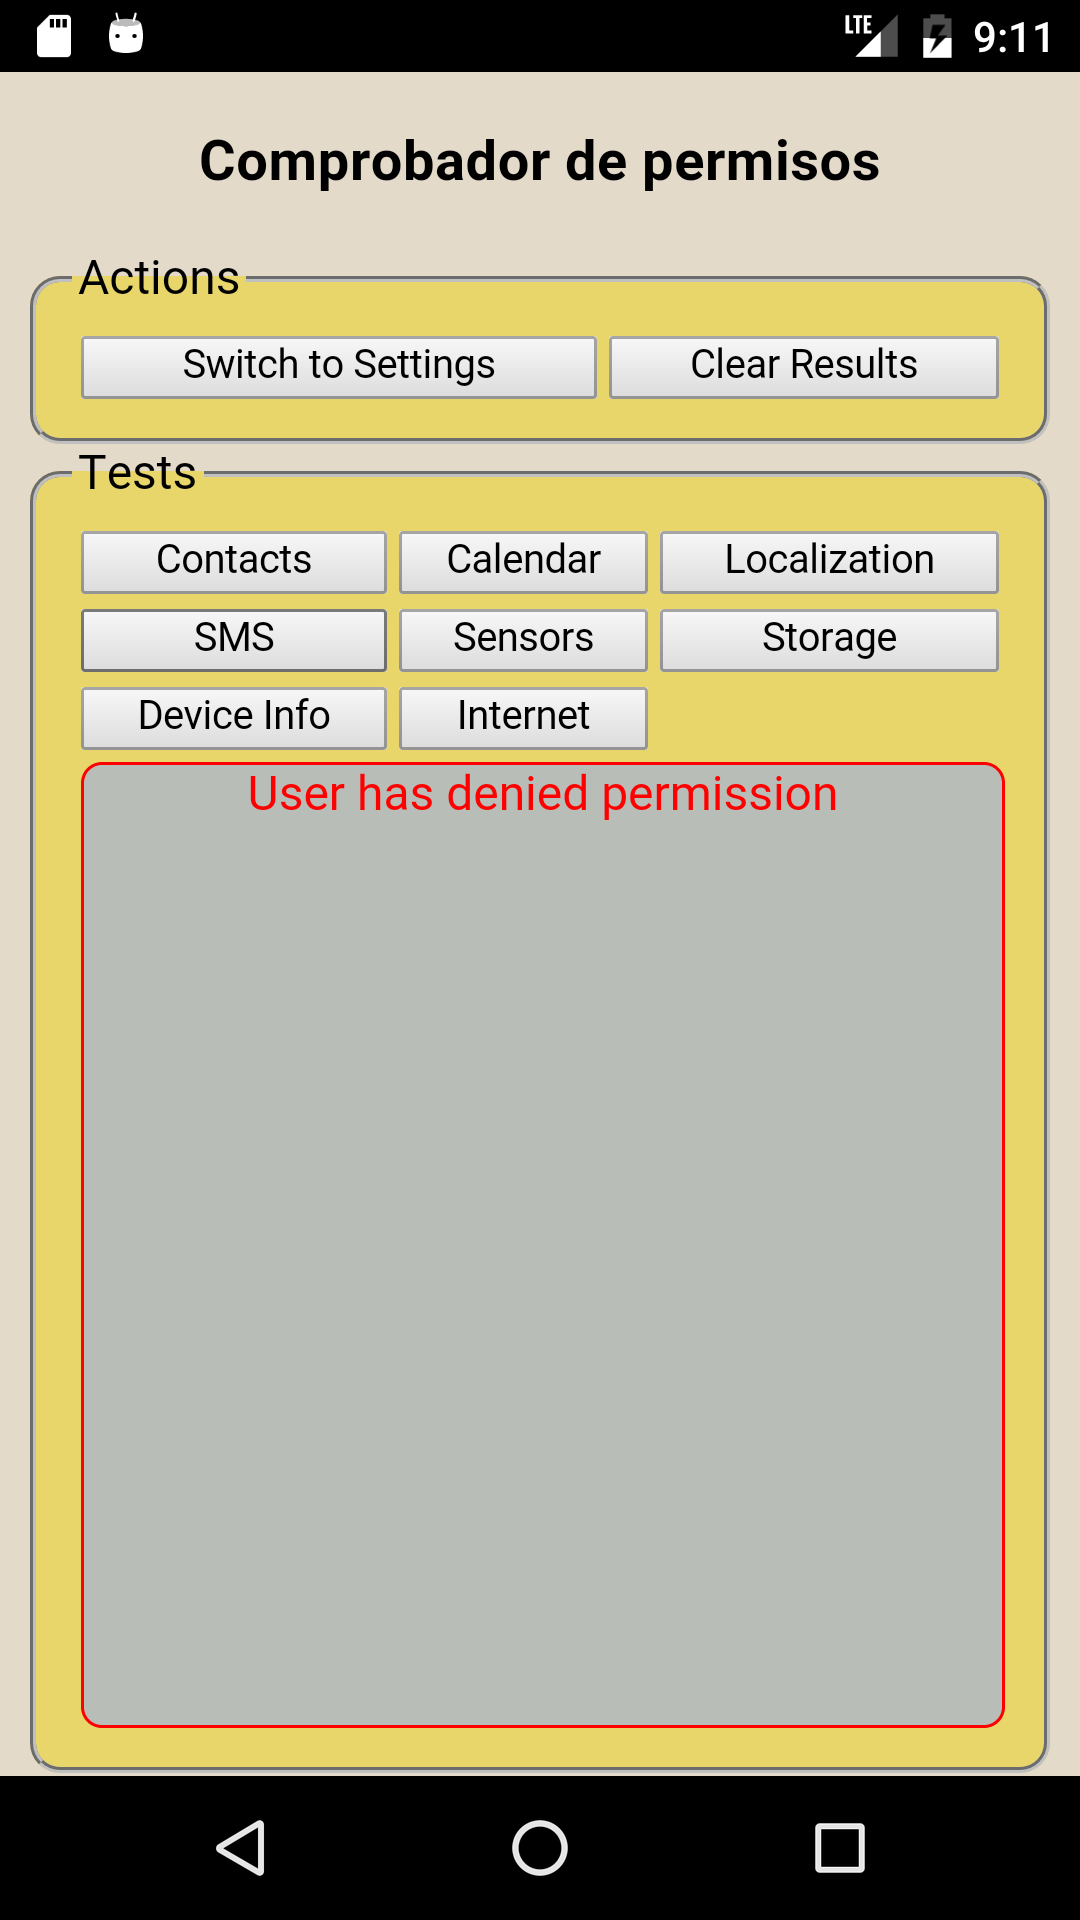
\includegraphics[width=\linewidth]{chapter5/without_sms}
		\caption{Sin permisos.}
		\label{fig:ch05:without_sms}
	\end{subfigure}
	\begin{subfigure}{.3\linewidth}
	    \centering
		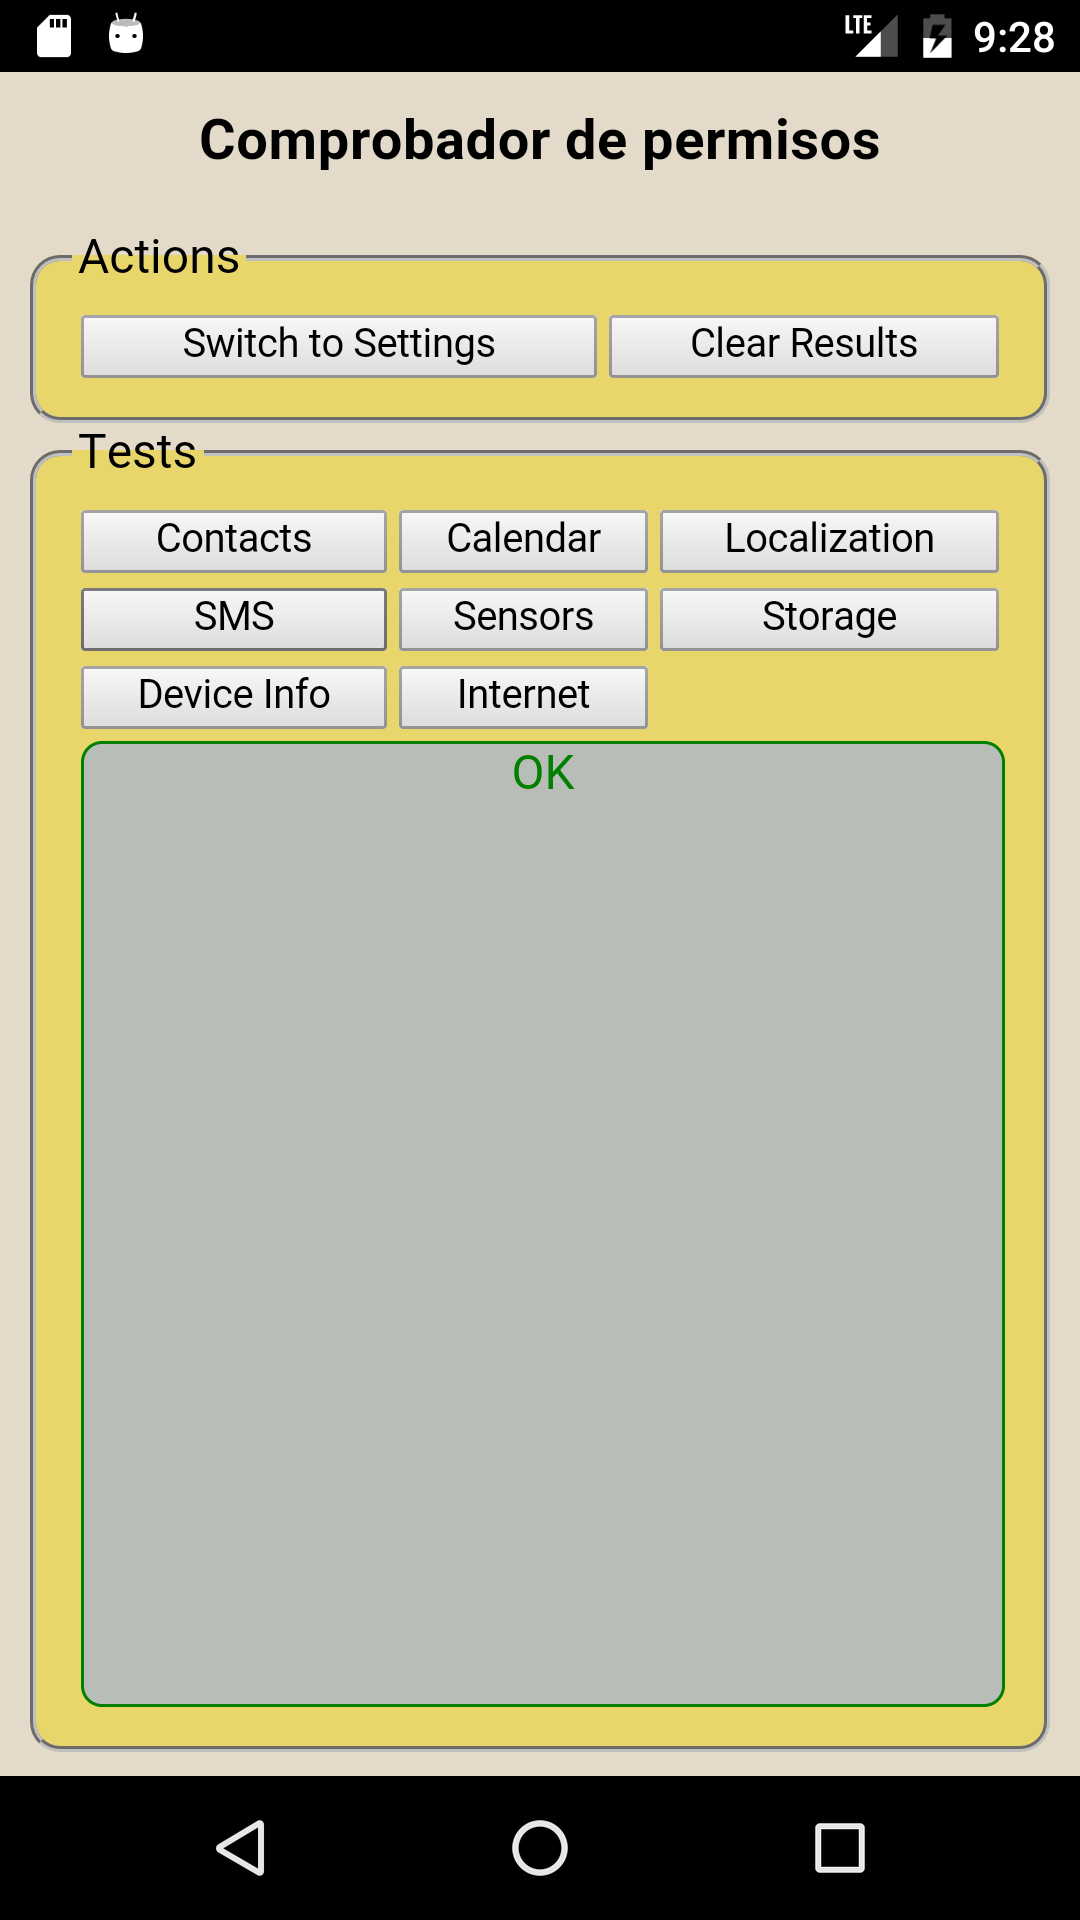
\includegraphics[width=\linewidth]{chapter5/success_sms}
		\caption{Con permisos.}
		\label{fig:ch05:with_sms}
	\end{subfigure}
	\caption{Testeando los mensajes SMS.}
	\label{fig:chapter05:sms_test}
\end{figure}
\subsection{Almacenamiento}
\begin{algorithm}
	\begin{algorithmic}[1]
		\STATE Se realiza una captura de la pantalla.
		\STATE Se guarda la captura en el dispositivo.
		\STATE Se imprime por consola el resultado del test.
	\end{algorithmic}
	\caption{Test de Almacenamiento.}\label{alg:chap5_test_storage}
\end{algorithm}
El presente test fue diseñado para probar el alcance de los permisos de escritura sobre el sistema de archivos que tiene cada plataforma. En la Figura \ref{fig:ch05:storage_fail} se observa el resultado del test cuando no se tiene el permiso correspondiente; mientras que en la Figura \ref{fig:ch05:storage_success} se observa el caso exitoso.\\

Para desarrollar el presente test se utilizó el \textit{plugin} \href{https://github.com/gitawego/cordova-screenshot}{cordova-screenshot (v. 0.1.5)} de Apache Cordova.\\

Finalmente, para correr el test, es necesario tener el permiso \texttt{Almacenamiento} para Android. Sin embargo, no es necesario tener permisos para correr el test en iOS.
\begin{figure}[hbtp]
   \centering
   	\begin{subfigure}{.3\linewidth}
		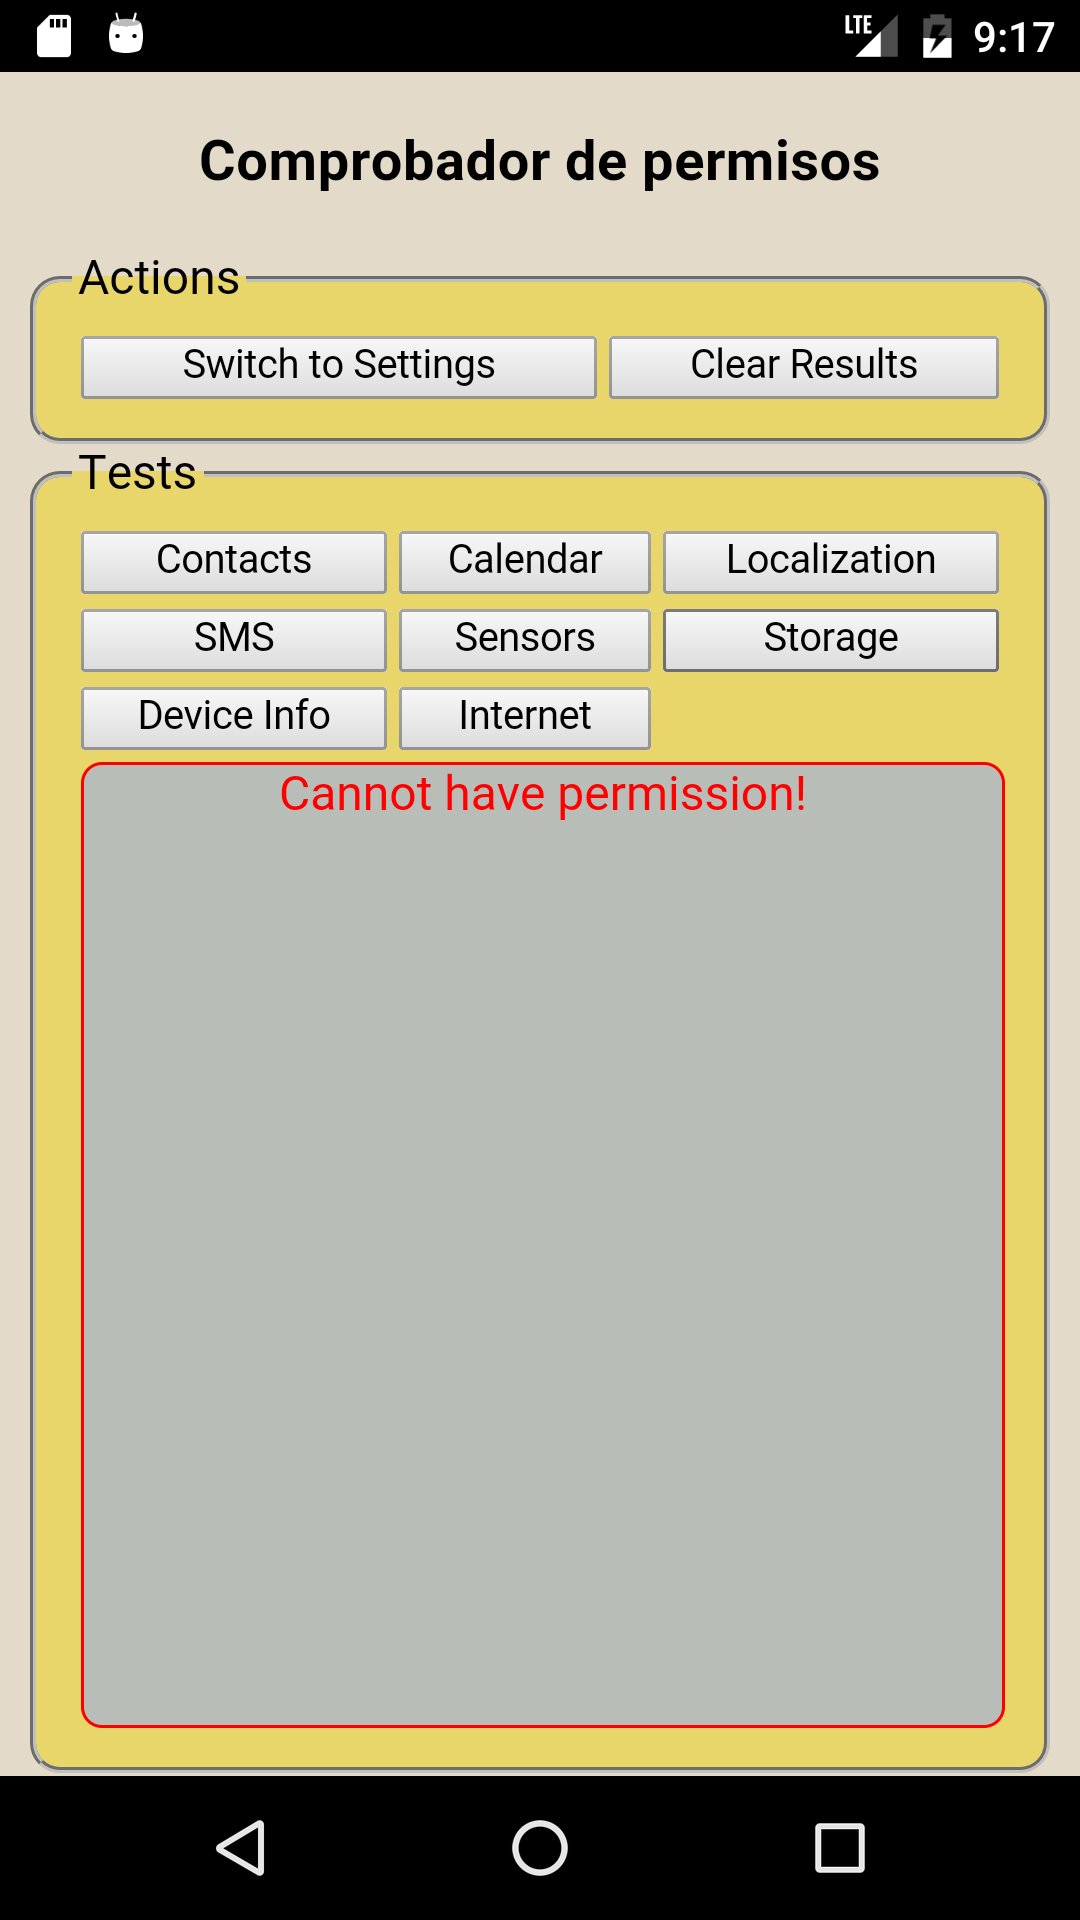
\includegraphics[width=\linewidth]{chapter5/storage_fail}
		\caption{Sin permisos.}
		\label{fig:ch05:storage_fail}
	\end{subfigure}
	\begin{subfigure}{.3\linewidth}
		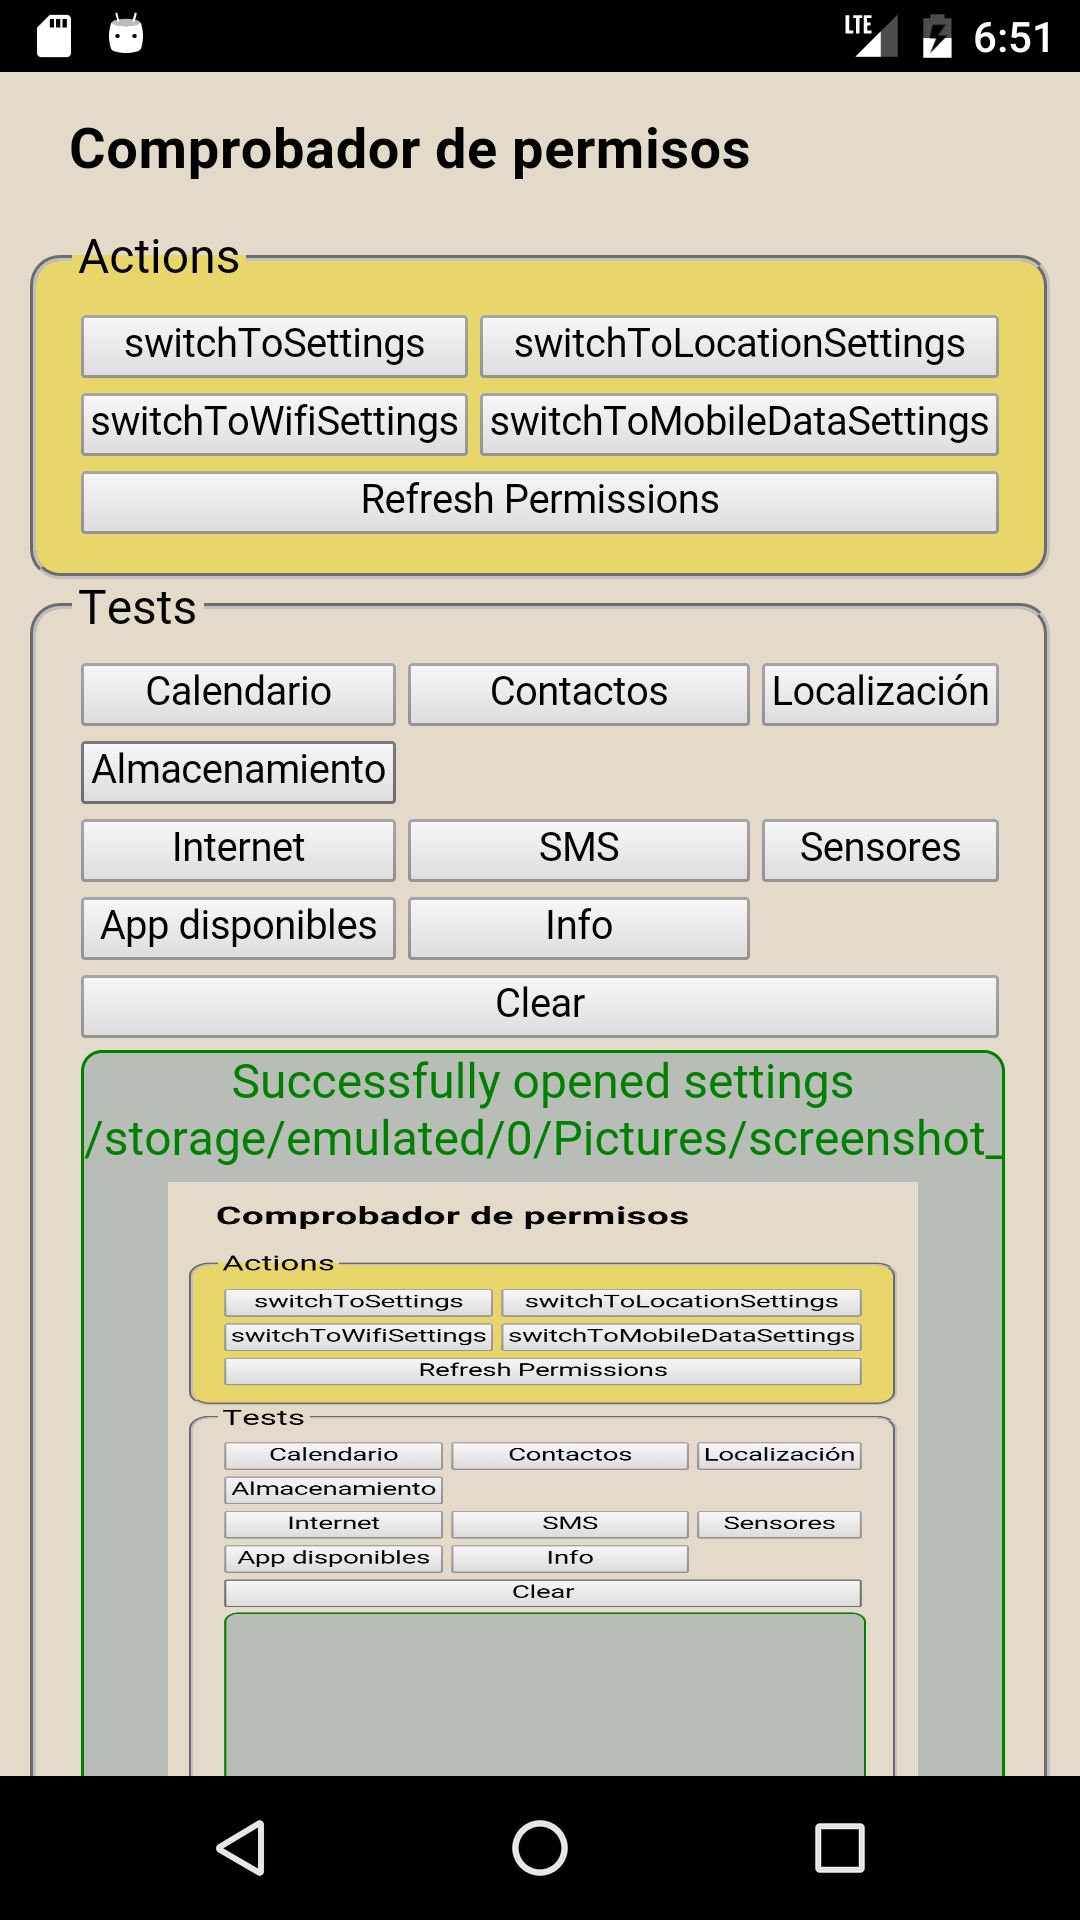
\includegraphics[width=\linewidth]{chapter5/storage_success}
		\caption{Con permisos.}
		\label{fig:ch05:storage_success}
	\end{subfigure}
	\caption{Testeando el almacenamiento del dispositivo.}
	\label{fig:ch05:storage_test}
\end{figure}
\subsection{Información del Dispositivo}
\begin{algorithm}
	\begin{algorithmic}[1]
		\STATE Se obtienen los datos del dispositivo.
		\STATE Se imprime por consola los datos obtenidos.
	\end{algorithmic}
	\caption{Test de Información del Dispositivo.}\label{alg:chap5_test_info}
\end{algorithm}
El objetivo de este test es obtener datos del dispositivo donde corre la aplicación. Entre otros datos, se obtiene la plataforma, modelo del dispositivo y su número de serie. En la Figura \ref{fig:ch05:device-info} se observan los datos obtenidos.\\

Para desarrollarlo se utilizó el \textit{plugin} \href{https://www.npmjs.com/package/cordova-plugin-device}{cordova-plugin-device (v.1.1.6)} de Apache Cordova.\\

Cabe aclarar que no fueron necesarios permisos en ninguna de las dos plataformas para poder correrlo.
\begin{figure}[hbtp]
   \centering
	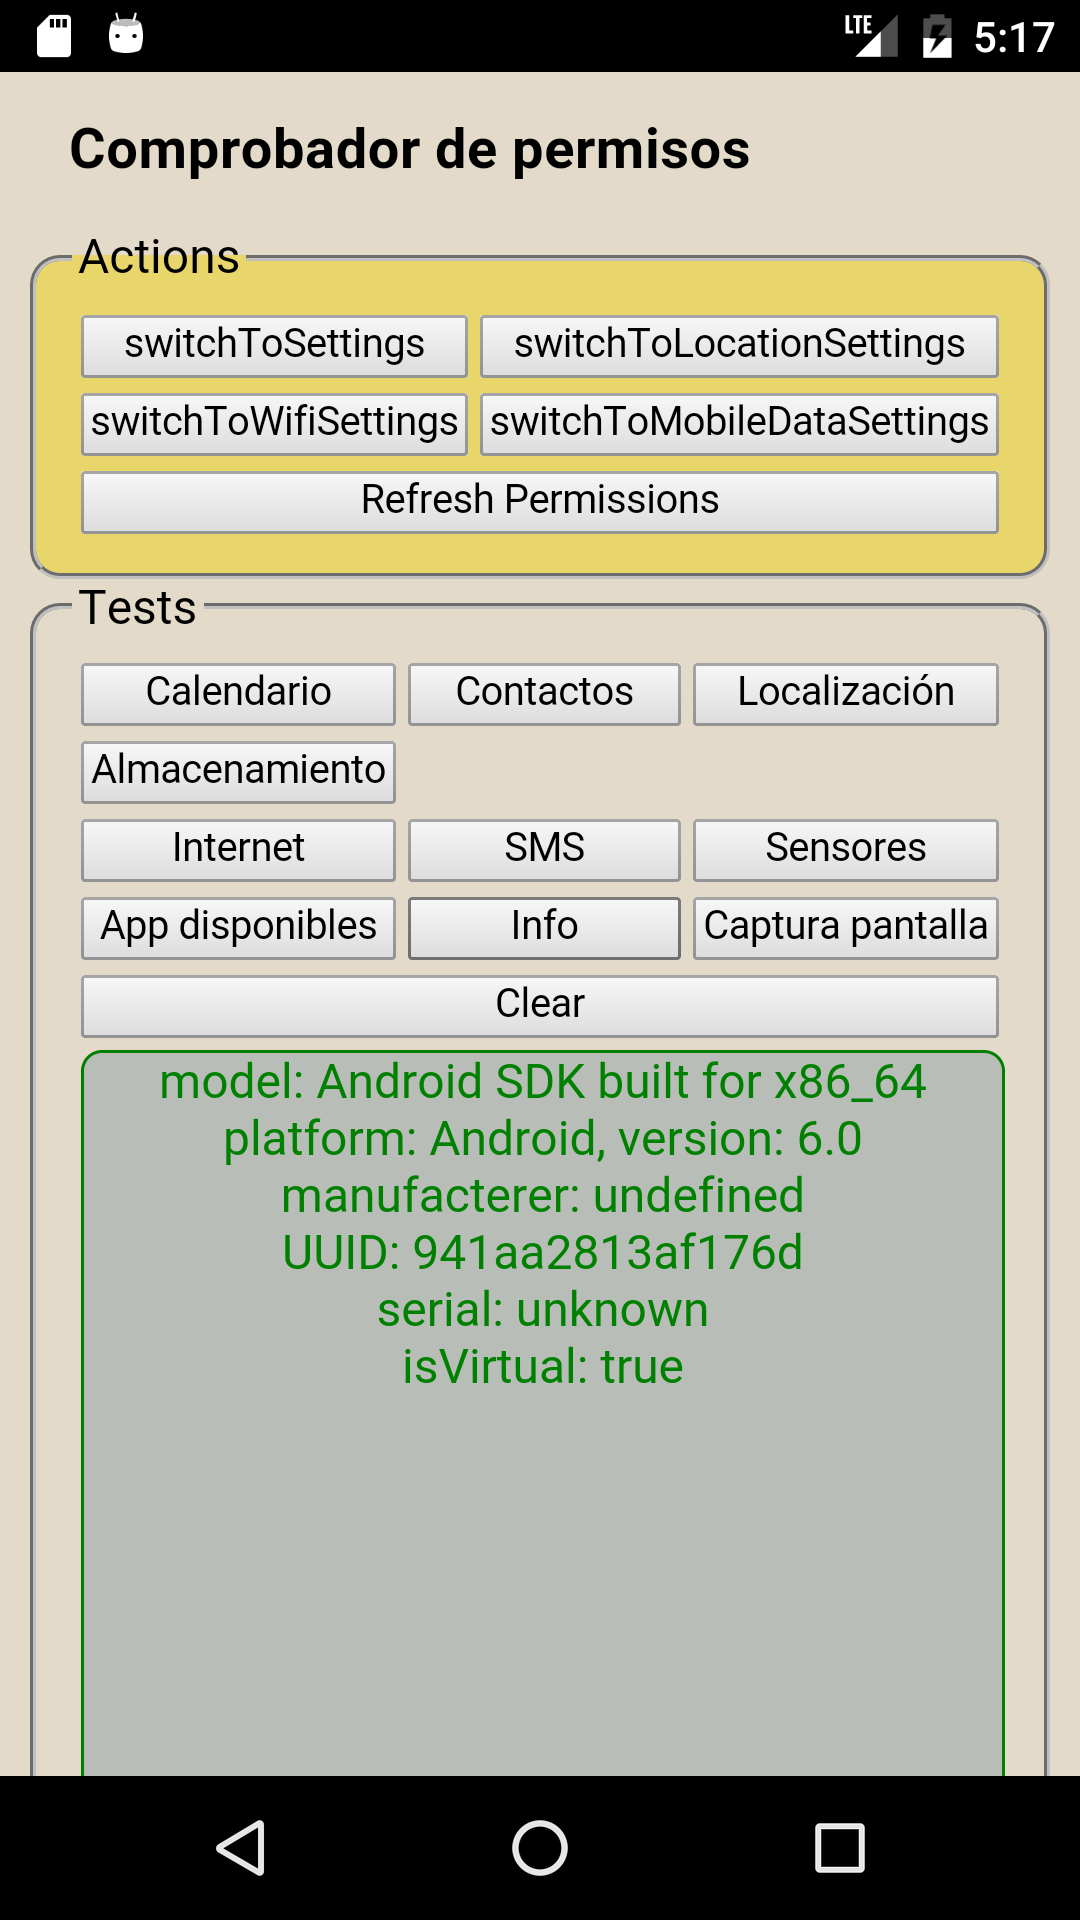
\includegraphics[width=0.3\linewidth]{chapter5/device_info}
	\caption{Testeando Información del Dispositivo.}
	\label{fig:ch05:device-info}
\end{figure}
\subsection{Sensores}
\begin{algorithm}
	\begin{algorithmic}[1]
		\STATE Se inicializa un \texttt{timer} con \texttt{5 seg} para detener las mediciones.
		\STATE Se inicia la medición del acelerómentro.
		\STATE Se inicia la medición del giroscopio.
		\STATE Se muestran los resultados en la consola.
	\end{algorithmic}
	\caption{Test de los Sensores.}\label{alg:chap5_test_sensors}
\end{algorithm}
El objetivo de este test es obtener datos de dos sensores del dispositivo: acelerómentro y giroscopio. Para ello, se configura un \texttt{timer}. Durante el tiempo que este activo, se tomarán distintos muestreos; y cuando ocurra el \emph{timeout} se mostrarán los datos en la consola de la aplicación. En la Figura \ref{fig:ch05:sensors_test} se observan los datos obtenidos.\\

Para desarrollar el presente test se utilizaron los \textit{plugins} \href{https://www.npmjs.com/package/cordova-plugin-device-motion}{cordova-plugin-device-motion} y \href{https://www.npmjs.com/package/cordova-plugin-gyroscope}{cordova-plugin-gyroscope}, de Apache Cordova.\\

Cabe aclarar que no fueron necesarios permisos en ninguna de las dos plataformas para poder correrlo.
\begin{figure}[tp]
    \centering
	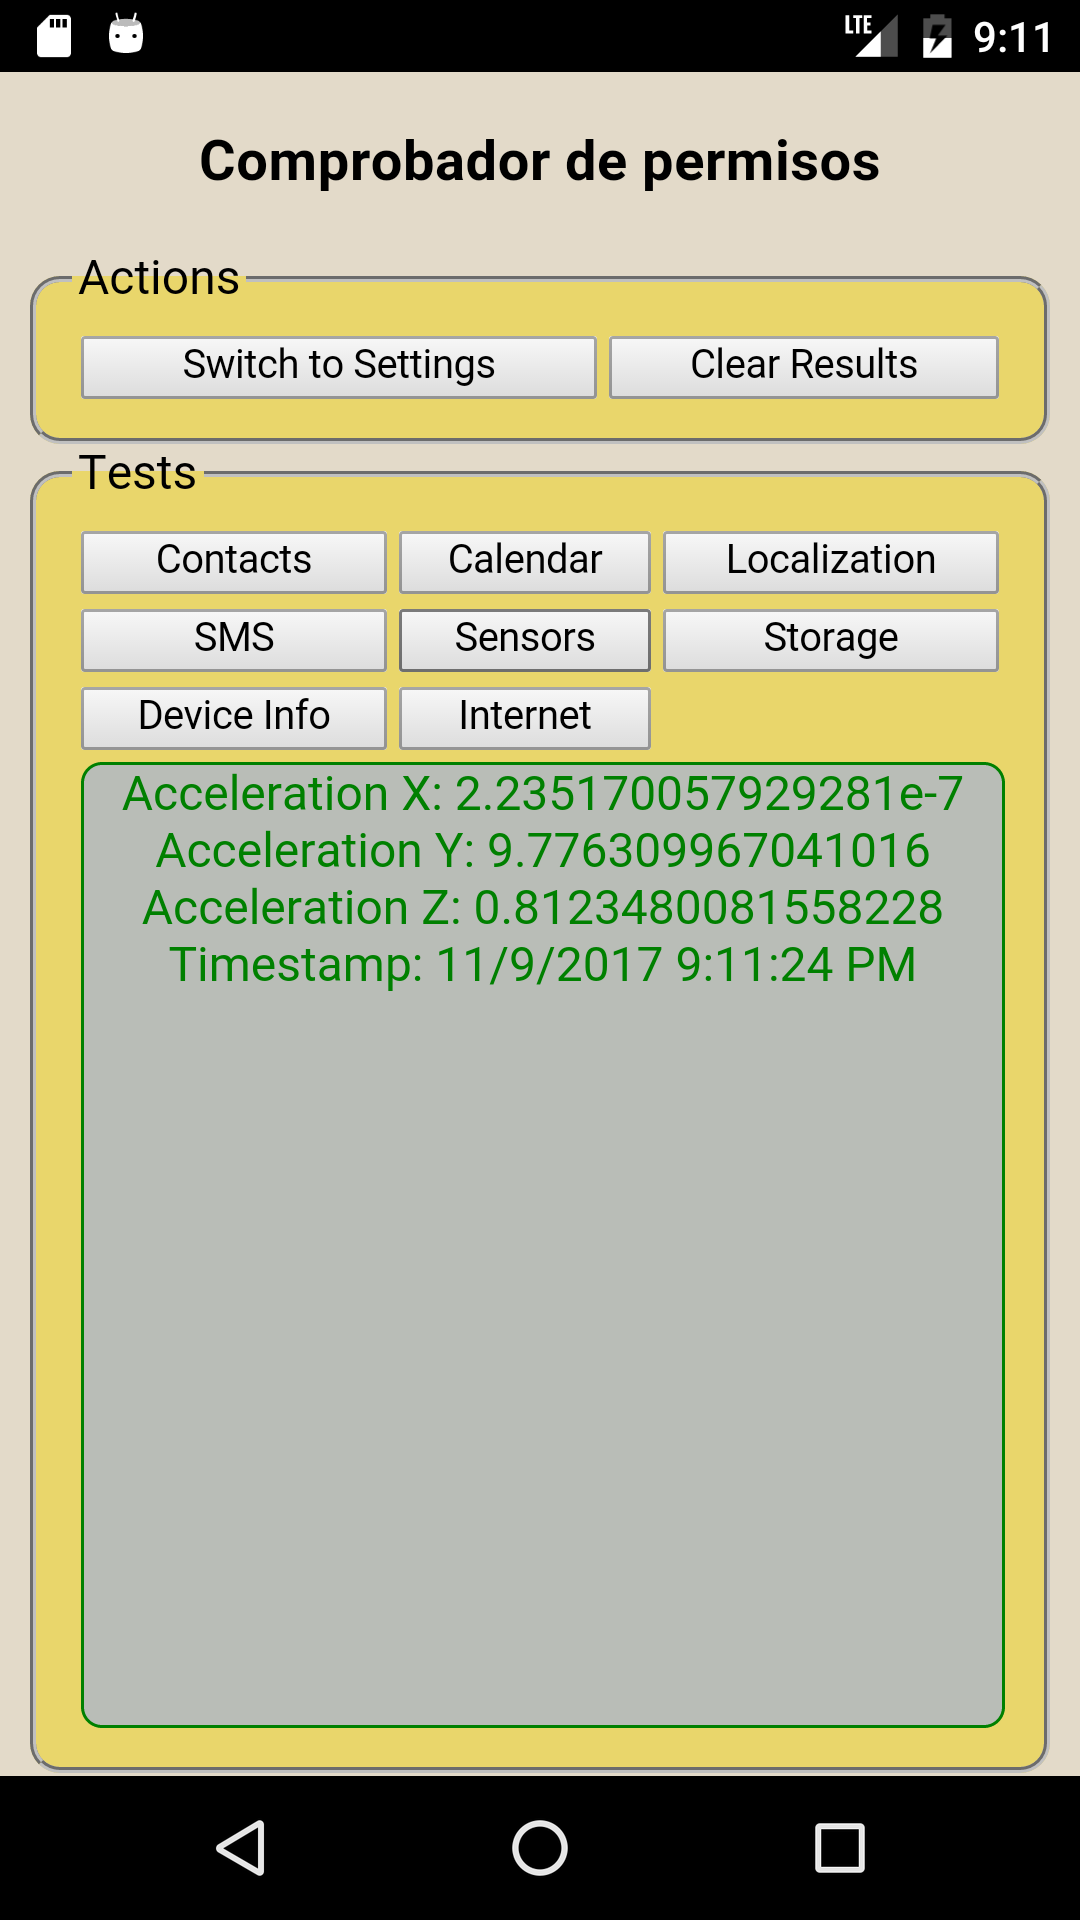
\includegraphics[width=.3\linewidth]{chapter5/sensors_success}
	\caption{Testeando los sensores.}
	\label{fig:ch05:sensors_test}
\end{figure}

\subsection{Internet}
\begin{algorithm}
	\begin{algorithmic}[1]
		\STATE Se realiza una consulta GET HTTP hacia \href{https://dcc.fceia.unr.edu.ar/sites/all/themes/birthofcool/images/logo-lcc.png}{logo del DCC}.
		\STATE Se decodifica la imagen (viene codificada en Base64).
		\STATE Se imprime por consola un \texttt{tag} \textless IMG\textgreater, cuyo \texttt{source} es el dato decodificado.
		\STATE Se realiza una consulta POST HTTP hacia \href{http://httpbin.org/post}{httpbin}.
		\STATE Se imprime por consola la respuesta.
	\end{algorithmic}
	\caption{Test de conexión a Internet.}\label{alg:chap5_test_internet}
\end{algorithm}
El objetivo del presente test es establecer una comunicación a través de Internet. Al momento de desarrollarlo, no se requirió de ningún \textit{plugin} de Apache Cordova.\\

En la Figura \ref{fig:ch05:fail_request} se observa el resultado del test cuando no se tiene conexión a Internet; mientras que en la Figura \ref{fig:ch05:success_request} se observa el caso de establecer una comunicación por Internet.\\

Cabe aclarar que, al ejecutarse el framework desde un emulador, para probar el acceso a Internet se habilitó/deshabilitó la Red Inalámbrica de la computadora donde se corrieron los emuladores.\\

Por último, no son necesarios permisos en ninguna de las dos plataformas para poder utilizar el presente test.
\begin{figure}[tp]
    \centering
    \begin{subfigure}{.35\linewidth}
		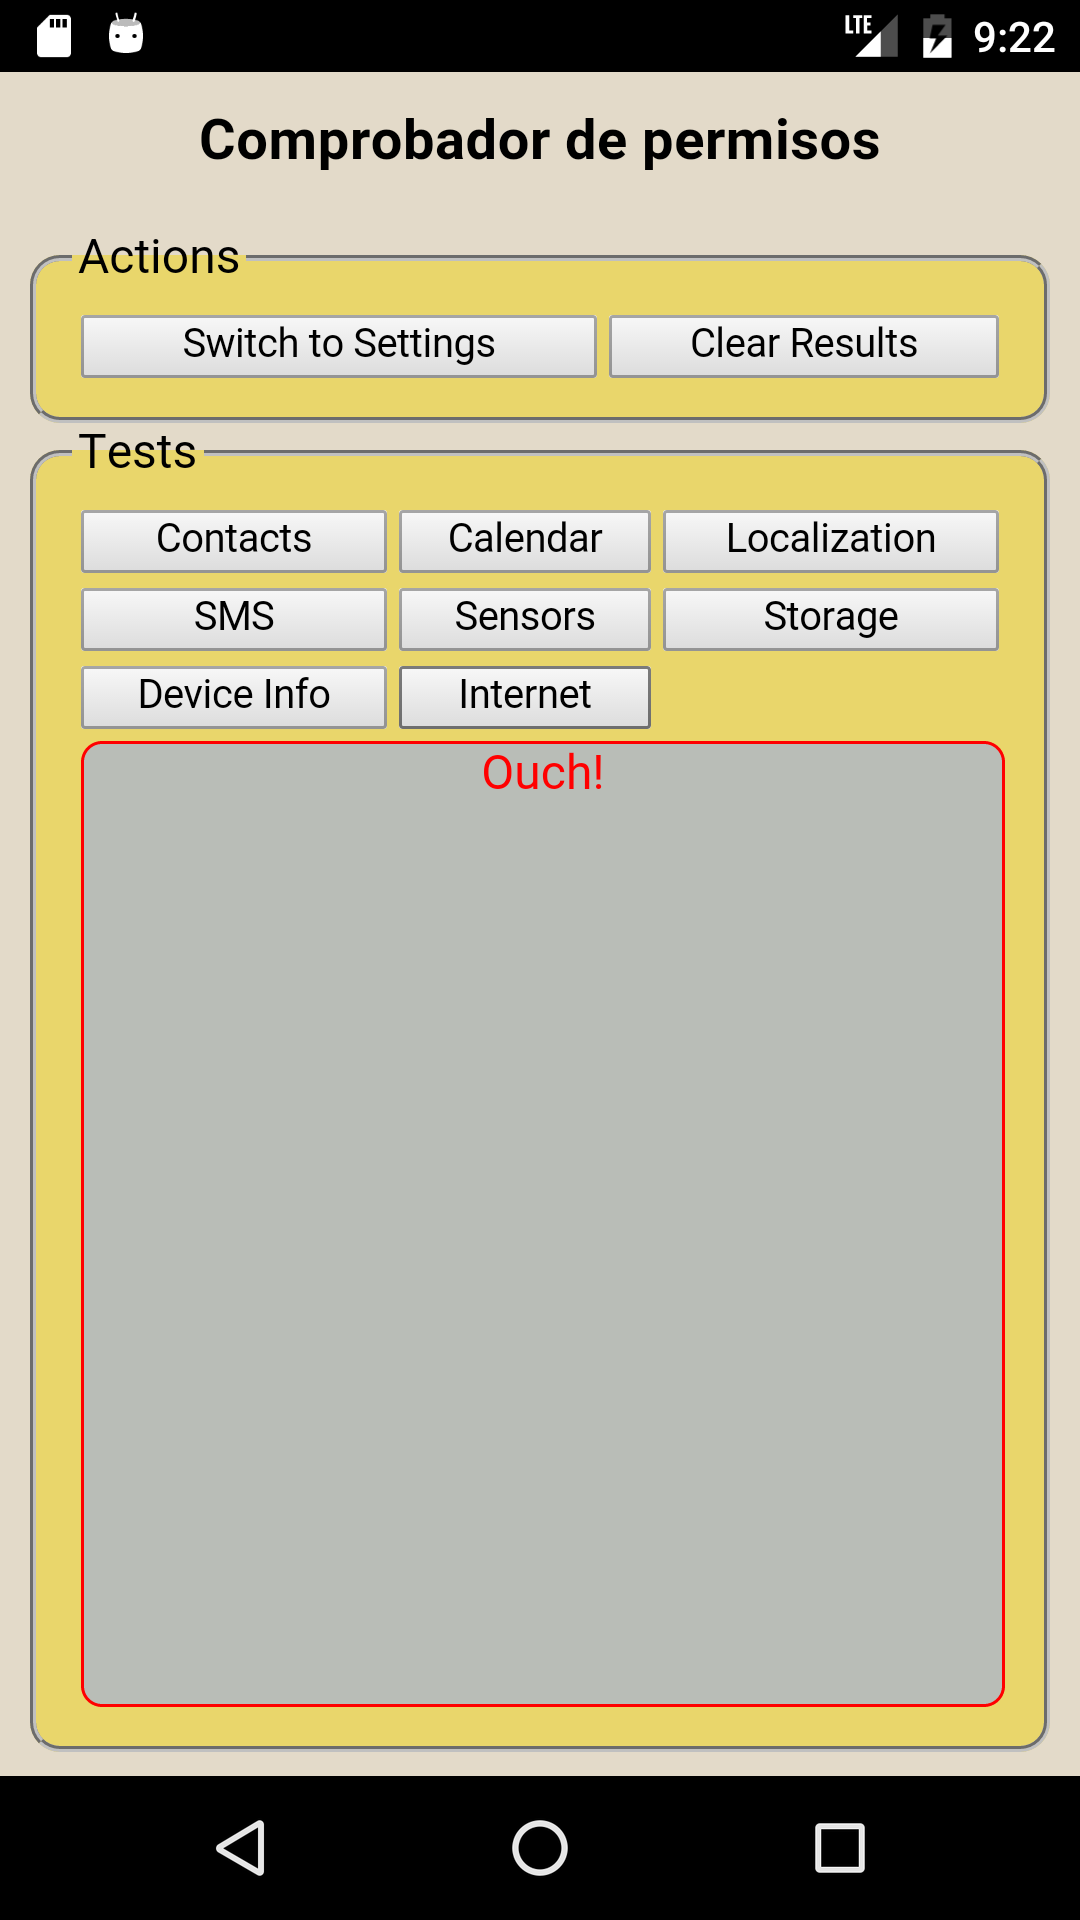
\includegraphics[width=\linewidth]{chapter5/fail_request}
		\caption{Sin conexión a Internet.}
		\label{fig:ch05:fail_request}
	\end{subfigure}
	\begin{subfigure}{.35\linewidth}
		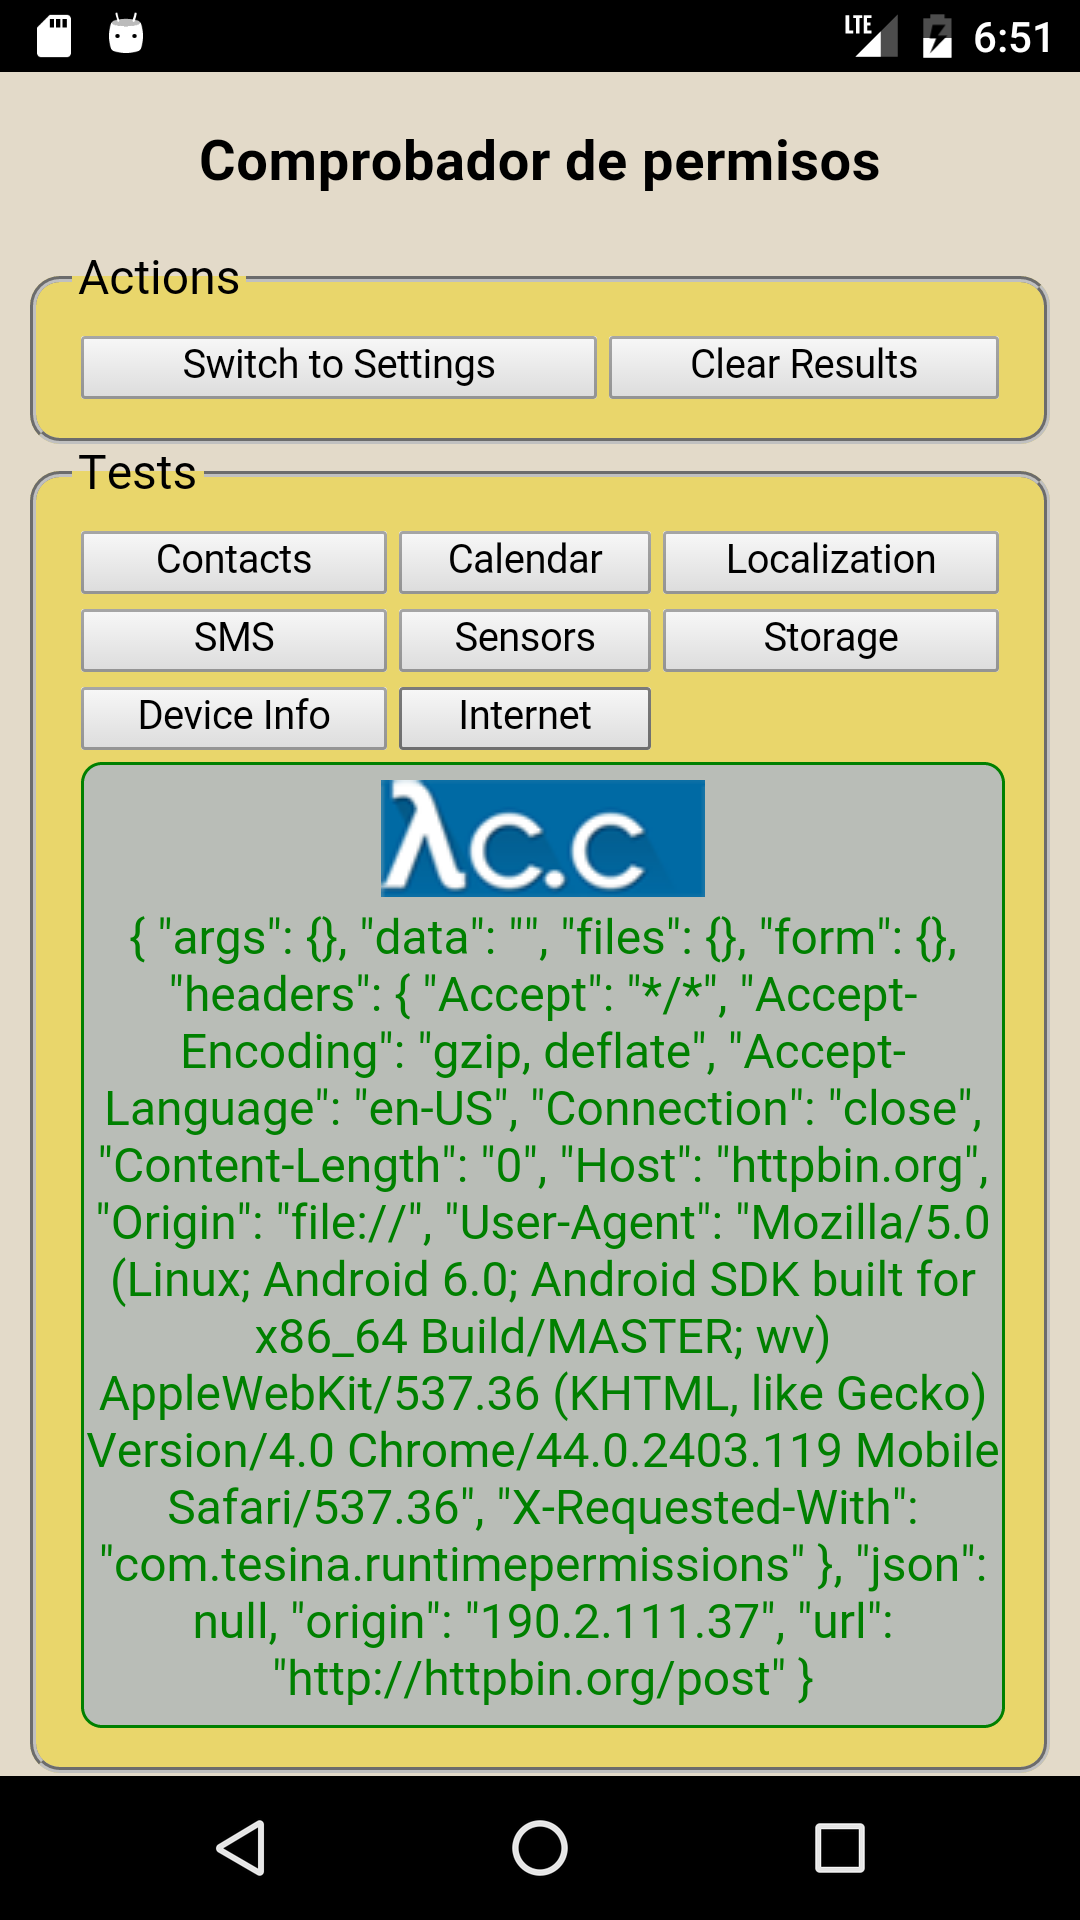
\includegraphics[width=\linewidth]{chapter5/success_request}
		\caption{Con conexión a Internet.}
		\label{fig:ch05:success_request}
	\end{subfigure}
	\caption{Testeando el acceso a Internet.}
	\label{fig:ch05:internet_test}
\end{figure}
\section{Resultados experimentales}
El \textit{framework} desarrollado en este trabajo tiene la capacidad de testear los componentes \emph{Contactos}, \emph{Calendario}, \emph{Geolocalización}, \emph{SMS}, \emph{Sensores}, \emph{Almacenamiento}, \emph{Información del dispositivo} y \emph{Acceso a Internet}, tal como se explicó en la Sección \ref{sec:main-view}.\\

Un primer resultado es poder clasificar los componentes testeados en cuatro clases, según requieran autorización del usuario para utilizarlos. Dichas clases son:
\begin{itemize}
    \item \underline{Clase A}: componentes que requieren autorización explícita en ambas plataformas para poder utilizar las funcionalidades que proveen;
    \item \underline{Clase B}: componentes que requieren autorización explícita solamente en Android;
    \item \underline{Clase C}: componentes que requieren autorización explícita solamente en iOS;
    \item \underline{Clase D}: componentes que no requieren autorización explícita para poder utilizar las funcionalidades que proveen.
\end{itemize}
Las clases son mutuamente excluyentes. Luego de correr los tests provistos por el \textit{framework}, se armó el Cuadro \ref{tab:ch03:permission-classification}. Cada test permitió clasificar a un componente presente en ambas plataformas.\\

A continuación, se detalla como están conformadas las clases.
\begin{table}[hbtp]
    \centering
	\begin{tabular}{c c c c}
		\hline
		\multicolumn{4}{c}{\emph{\textbf{Permisos}}} \\
		\emph{Clase A} 	& \emph{Clase B}	 & \emph{Clase C}    & \emph{Clase D}\\ \hline \hline
    Contactos    & -    & -    & -\\
    Calendario    & -    & -    & -\\
    Geolocalización    & -    & -    & -\\
    -    & SMS\tablefootnote{Aplica solamente al envío de mensajes.}    & -    & -\\
    -    & Almacenamiento    & -    & -\\
    -    & -    & -    & Sensores\\
    -    & -    & -    & Información del dispositivo\\
    -    & -    & -    & Acceso a Internet\\ \hline
	\end{tabular}
	\caption{Clasificación de permisos según si requieren autorización.}
	\label{tab:ch03:permission-classification}
\end{table}
\subsection{Clase A}
Los componentes que conforman esta clase son \emph{Contactos}, \emph{Calendario} y \emph{Geolocalización}. La característica común entre ellos es que requieren autorización explícita del usuario para interactuar con ellos. Si el usuario deniega el correspondiente permiso, no se puede acceder a ninguna funcionalidad del componente.\\
El primer componente a analizar es \emph{Contactos}. En Android, requiere el permiso \textit{peligroso} llamado Contacto y en iOS requiere el permiso llamado con el mismo nombre. En ambas plataformas, los dos permisos abarcan las mismas funcionales: permiten crear un contacto, borrarlo, editarlo y obtener un listado de todos los contactos presentes en el dispositivo.\\

Luego, se continúa analizando el componente \emph{Calendario}. En Android permite administrar todo lo relacionado con los eventos: crear un evento, modificarlo y eliminarlo. Además, permite administrar varios calendarios, permitiendo por ejemplo, tener un calendario que contenga los eventos laborales y otro con los eventos personales. En iOS, estas funcionalidades están separadas en dos componentes: \emph{Calendarios} y \emph{Recordatorios}. Cada uno de ellos tiene su permiso que lo regula. Sin embargo, el test presente en el \textit{framework} prueba solamente el componente \emph{Recordatorios}. Para poder correrlo, es necesario tener el permiso Recordatorios. Por otra parte, en Android, el permiso \textit{peligroso} que regula las funcionalidades mencionadas anteriormente, se llama Calendario.\\

A continuación se analiza el último componente de esta clase, llamado \emph{Geolocalización}. En ambas plataformas, provee el acceso a la ubicación del dispositivo, ya sea la ubicación precisa (GPS) o la aproximada (WIFI/Móvil). Tanto en Android como en iOS, el permiso que regula dichas funcionalidades se llama Localización.
\subsection{Clase B}
Esta clase está compuesta por los componentes \emph{SMS} y \emph{Almacenamiento}. Ellos tienen en común que para utilizar sus funcionalidades no requieren permisos en iOS. Sin embargo, necesitan autorización explícita en Android.\\

Se comenzará el análisis por el componente \emph{SMS}. Sus funcionalidades son: enviar un mensaje, eliminarlo, obtener los mensajes entrantes y obtener la lista de todos los mensajes, ya sean recibidos o enviados. Sin embargo, el test presente en el \textit{framework} solamente prueba el envío de mensajes, ya que en iOS, a partir de la version 8 no permite acceder al resto de las funcionalidades desde una aplicación de terceros (es decir, no nativa) \cite{foda, foda2}. En cambio, Android permite acceder a todas las funcionalidades mencionadas; y se pueden acceder teniendo el permiso \textit{peligroso} llamado SMS.\\

Finalmente, se hablará sobre el componente \emph{Almacenamiento}. El permiso que regula al componente en Android tiene su mismo nombre. Dicho permiso resguarda las funcionalidades que permiten leer y escribir la tarjeta SD. El test presente en el \textit{framework} solamente prueba escribir en el sistema de archivos.
\subsection{Clase C}
Los componentes que agrupa la presente clase son aquellos que requieren algún permiso en iOS y no requieren permisos en Android para poder utilizar sus funcionalidades.\\

Cabe aclarar que la presente clase es puramente teórica, ya que ninguno de los componentes analizados pertenecen a ella. Sin embargo, se mantuvo en el informe ya que es posible que exista algún componente en dicha clase, que pueda ser descubierto en futuras versiones del \textit{framework}.
\subsection{Clase D}
La presente clase agrupa componentes que no requieren autorización explícita del usuario para utilizar las funcionalidades que brindan. Sus miembros son \emph{Información del dispositivo}, \emph{Sensores} y \emph{Acceso a Internet}.\\

Como se explica en la sección \ref{ch03-permisos}, si una aplicación requiere algún permiso asociado a un componente de esta clase, el sistema operativo se lo otorga al momento de instalación. Es por ello que los miembros de esta clase pueden ser potencialmente peligrosos respecto de la privacidad del usuario, ya que exponen medios o información que, combinadas con otros componentes, pueden violar dicha privacidad.\\

Por ejemplo, supongamos que se tiene instalada una aplicación maliciosa de administración de contactos. Supongamos también, para simplificar, que requiere solamente de dos componentes: Contactos y Acceso a Internet. Según el Cuadro \ref{tab:ch03:permission-classification}, al usuario se le requeriría explícitamente el permiso \emph{Contactos}. Sin embargo, dicha aplicación maliciosa obtiene el permiso correspondiente a Acceso a Internet sin que el usuario sea notificado. Ergo, ¡puede robar todos los contactos!\\

Empecemos el análisis de los miembros de la clase. El primer componente nos brinda datos relacionados al dispositivo en el cual se está corriendo la aplicación. Especifica el modelo del dispositivo, el cual es establecido por el fabricante del dispositivo y puede ser diferente en todas las versiones del mismo producto. También se puede obtener información relacionada a la plataforma del dispositivo: nombre, versión, quién lo manufacturó, su UUID\footnote{Del inglés Universally Unique Identifier. Es un numero de 128 bits que identifica al dispositivo biunívocamente.} y si es emulado o no.\\

Luego, se continúa con el componente \emph{Sensores}. Dicho componente controla el acceso a los sensores del dispositivo. El test presente en el \textit{framework} recolecta datos de dos sensores: el acelerómentro y el giroscopio. Con los datos obtenidos, se podrían calcular varios movimientos del dispositivo, tales como inclinación, vibración, rotación o balanceo.\\

El último componente de esta clase es el que nos provee acceso a Internet. En la actualidad, son muchas las aplicaciones móviles que utilizan Internet. Según el ranking confeccionado por \cite{BOA}, las 10 aplicaciones más populares utilizan Internet. El test permite realizar una petición GET y una petición POST sin notificar al usuario. Esto es potencialmente muy peligroso ya que una aplicación maliciosa puede enviar y recibir datos sin que el usuario lo note. Por ejemplo, supongamos que tenemos una aplicación maliciosa que nos oficia de navegador GPS. Supongamos también que el usuario le otorga el permiso para utilizar el GPS. Sin embargo, dicha aplicación podría enviar a través de Internet todas las rutas realizadas por el usuario, sin que el mismo sea notificado.